\documentclass[conference]{IEEEtran}
\IEEEoverridecommandlockouts
% The preceding line is only needed to identify funding in the first footnote. If that is unneeded, please comment it out.
\usepackage{cite}
\usepackage{amsmath,amssymb,amsfonts}
\usepackage{algorithmic}
\usepackage{graphicx}
\usepackage{textcomp}
\usepackage{xcolor}
\def\BibTeX{{\rm B\kern-.05em{\sc i\kern-.025em b}\kern-.08em
    T\kern-.1667em\lower.7ex\hbox{E}\kern-.125emX}}
\begin{document}

\title{Studi Komparasi Performa Algoritma \textit{Supervised-Learning} dalam Klasifikasi Multidataset\\
}

\author{\IEEEauthorblockN{I Gusti Ngurah Ryo Aditarta}
\IEEEauthorblockA{\textit{Fakultas Ilmu Komputer} \\
\textit{Universitas Brawijaya}\\
Malang, Indonesia \\
ryoaditarta@student.ub.ac.id}

\and

\IEEEauthorblockN{2\textsuperscript{nd} Dian Pandu Syahfitra}
\IEEEauthorblockA{\textit{Fakultas Ilmu Komputer} \\
\textit{Universitas Brawijaya}\\
Malang, Indonesia \\
dianpandu@student.ub.ac.id}

\and

\IEEEauthorblockN{3\textsuperscript{rd} Rayhan Egar Sadtya Nugraha}
\IEEEauthorblockA{\textit{Fakultas Ilmu Komputer} \\
\textit{Universitas Brawijaya}\\
Malang, Indonesia \\
rayhanegar@student.ub.ac.id}

\and

\IEEEauthorblockN{4\textsuperscript{th} Ahmad Zaki}
\IEEEauthorblockA{\textit{Fakultas Ilmu Komputer} \\
\textit{Universitas Brawijaya}\\
Malang, Indonesia \\
ahmadzaki12@student.ub.ac.id}

\and

\IEEEauthorblockN{5\textsuperscript{th} Muhammad Arya Ghifari}
\IEEEauthorblockA{\textit{Fakultas Ilmu Komputer} \\
\textit{Universitas Brawijaya}\\
Malang, Indonesia \\
aryaghifary07@student.ub.ac.id}

\and
\IEEEauthorblockN{6\textsuperscript{th} Arion Syemael Siahaan}
\IEEEauthorblockA{\textit{Fakultas Ilmu Komputer} \\
\textit{Universitas Brawijaya}\\
Malang, Indonesia \\
siahaanarion@student.ub.ac.id}
}

\maketitle

\begin{abstract}
    Machine Learning (ML) is a cornerstone technology advancing various aspects of human life, focusing on developing algorithms that enable systems to learn from data and make predictions or 
    decisions without explicit programming. A key aspect of ML is supervised learning, where models learn from input-output pairs to predict or classify new data. This paper aims to address the challenge of 
    selecting appropriate classification methods by comparing various techniques from the literature.

    Datasets used include Spaceship Titanic, Bank Churn, Horse Health, and Keep-it-Dry, each chosen for their diverse features and predictive challenges. Preprocessing steps involve data encoding, 
    scaling, and handling missing values. Supervised learning algorithms explored are CatBoost, AdaBoost, LightGBM, and ensemble methods like stacking and K-Nearest Neighbor (KNN). Hyperparameter 
    optimization techniques such as GridSearchCV and Optuna are employed to enhance performance. Evaluation metrics include confusion matrix, recall, precision, accuracy, F1-score, AUC-ROC, and cross-validation.

    Results indicate that tree-based classifiers like LightGBM, CatBoost, and XGBoost generally perform well across different datasets, achieving higher accuracy and better generalization. 
    However, linear classifiers like Ridge Classifier and Logistic Regression also show competitive performance, especially in stability and reliability on test data, when combined with appropriate preprocessing techniques.

    In conclusion, this study underscores the importance of proper data preprocessing, the effectiveness of Principal Component Analysis (PCA) in improving model generalization, and the critical 
    role of hyperparameter tuning in developing robust ML models. The insights from this comparative analysis can guide practitioners in selecting and fine-tuning classification algorithms for varied predictive tasks.
\end{abstract}

\begin{IEEEkeywords}
Supervised Machine Learning, Classification Algorithms, Supervised Machine Learning Comparative Study
\end{IEEEkeywords}

\section{Introduction}
Pembelajaran Mesin (ML) telah menjadi salah satu fondasi teknologi yang mendukung kemajuan teknologi dalam berbagai aspek kehidupan manusia \cite{b2}. 
Sebagai cabang dari kecerdasan buatan (AI), ML bertujuan untuk mengembangkan algoritma dan model komputasional yang memungkinkan sistem untuk belajar dari data dan membuat 
prediksi atau keputusan tanpa perlu diprogram secara eksplisit \cite{b1}.

Salah satu aspek penting dari ML adalah supervised control, di mana model diberikan pasangan input-output dalam data pelatihan untuk mempelajari 
hubungan antara mereka \cite{b1}. Dengan menggunakan metode ini, model dapat melakukan prediksi atau klasifikasi pada data baru berdasarkan 
pembelajaran dari data pelatihan yang ada \cite{b1}.

Klasifikasi dengan supervised learning adalah salah satu teknik yang paling fundamental dan sering digunakan \cite{b1}. Dengan memanfaatkan dataset yang telah dilabeli, 
model dilatih untuk mengenali pola dan membuat prediksi yang akurat terhadap data baru \cite{b2}. Namun, dalam menghadapi berbagai tugas klasifikasi, peneliti dan praktisi ML 
seringkali dihadapkan pada tantangan dalam memilih metode yang paling sesuai untuk kasus tertentu \cite{b1}.

Paper ini dibuat bertujuan untuk menjawab tantangan tersebut dengan melakukan studi perbandingan terhadap berbagai metode klasifikasi yang telah diusulkan dalam literatur ilmiah \cite{b3}. 
Dengan menggunakan referensi dari jurnal-jurnal terkemuka, kami mengumpulkan berbagai pendekatan klasifikasi dengan supervised yang memiliki keunggulan dan kelemahan masing-masing \cite{b3}.

\section{Algoritma Klasifikasi Supervised Learning}

\subsection{K-Nearest Neighbors (KNN)}

Algoritma klasifikasi \textit{nearest neighbors} seperti KNN merupakan salah satu algoritma dasar nonparametrik 
dalam pembelajaran mesin. Hal ini didasarkan pada \textit{rationale} di mana fitur yang digunakan untuk 
mendeskripsikan label sebuah \textit{domain point} memiliki relevansi dengan \textit{domain point} lain dalam sisi 
\textit{proximity} \cite{b4, b5}. Dalam implementasinya, KNN banyak digunakan dalam permasalahan 
klasifikasi dengan domain pengetahuan yang terdefinisi dan diketahui dengan baik, 
seperti klasifikasi tumor otak \cite{b6}, klasifikasi tingkat keparahan Covid-19 \cite{b7}, maupun prognosis kanker \cite{b8}.

Secara prinsip, nilai parameter $k$ yang merepresentasikan banyaknya \textit{domain point} yang digunakan 
dalam penentuan label serta metode perhitungan jarak merupakan konsiderasi utama. Nilai $k$ yang
terlalu kecil memberikan model yang kompleks dan kurang mampu mengakomodasi \textit{unseen data}, sedangkan 
nilai $k$ yang terlalu besar memberikan model yang terlalu sederhana untuk secara akurat 
mengklasifikasikan suatu \textit{domain point} \cite{b9}. Beberapa teknik, seperti \textit{normalized class coherence}, 
\textit{change-based KNN}, \textit{variable selection} dan \textit{weighting}, maupun normalisasi L1 dan LPP dapat digunakan untuk 
memberikan estimasi yang lebih baik \cite{b10,b11,b12}. Selain itu, pilihan perhitungan jarak antara domain point 
dalam proses pembelajaran model seperti Euclidean ``\eqref{euclidean}'', Manhattan ``\eqref{manhattan}'', maupun Minkowski ``\eqref{minkowski}'' untuk pemetaan label kelas 
juga perlu untuk diperhatikan.

\begin{equation}
    d(x, y)=\sqrt{\sum_{i=1}^{n} (y_i - x_i)^2} \label{euclidean}
\end{equation}

\begin{equation}
    d(x,y) = \sum_{i=1}^{n}|x_i - y_i| \label{manhattan}
\end{equation}

\begin{equation}
    d(x, y) = (\sum_{i=1}^{n} |x_i - y_i|^p)^{\frac{1}{4}} \label{minkowski}
\end{equation}

\subsection{Ridge Classifier (RC)}

Algoritma klasifikasi \textit{Ridge Classifier} (RC) dikembangkan dari algoritma \textit{Ridge Regression} yang mengkombinasikan 
\textit{learning rule} \textit{Regularized Learning Minimization} (RLM) dengan regresi \textit{linear ordinary least squares} [1]. 
Algoritma RC melakukan \textit{class labelling} berdasarkan tanda/\textit{sign} dari suatu \textit{data point} (positif atau negatif). 
Penggunaan fungsi regularisasi, seperti regularisasi L2/Tikhonov ``\eqref{l2_norm}'' ``\eqref{tikhonov}'' pada algoritma klasifikasi memberikan model yang lebih “stabil” 
dan mencegah terjadinya \textit{overfitting} \cite{b4, b5}. Dibandingkan dengan regresi linear, algoritma RC akan meminimalisasi nilai 
koefisien $w$ untuk masing-masing fitur, memberikan model dengan kemampuan generalisasi yang baik terhadap \textit{unseen data}. Dengan demikian, fungsi
yang digunakan dalam RC dapat didefinisikan secara formal pada ``\eqref{ridgeregression}''.

\begin{equation}
    ||w|| = \sqrt{\sum_{i=1}^{d} w_i^2} \label{l2_norm}
\end{equation}

\begin{equation}
    \arg min _{w}(L_s(w) + \lambda ||w||^2) \label{tikhonov}
\end{equation}

\begin{equation}
    \arg min_{w \in R^d} (\lambda||w||^2 + \frac{1}{m}\sum_{i=1}^{m}(<w, x_i> - y_i)^2) \label{ridgeregression}
\end{equation}

Dalam melakukan proses pembelajaran model, parameter regularisasi menjadi konsiderasi utama. Semakin kecil nilai, nilai 
koefisien $w$ akan semakin kecil, memberikan model dengan generalisasi yang baik namun dengan potensi \textit{underfitting}. 
Nilai $\alpha$ yang semakin besar akan meminimalisasi efek regularisasi, memberikan model dengan kompleksitas yang lebih tinggi 
namun dengan potensi \textit{overfitting} untuk \textit{unseen data}. Selain dengan menggunakan \textit{cross-validation} untuk \textit{hyperparameter tuning}, teknik seperti 
\textit{fractional ridge regression} \cite{b13} dengan memanfaatkan rasio L2-norm antara \textit{regularized} dan \textit{normal coefficients} dapat membantu menemukan 
nilai $\alpha$ yang optimal.

\subsection{Logistic Regression (LR)}

\textit{Logistic Regression} (LR) merupakan algoritma klasifikasi yang didefinisikan secara formal sebagai komposisi fungsi 
sigmoid ``\eqref{sigmoid}''terhadap suatu fungsi regresi linear untuk membuat kelas hipotesis ``\eqref{logreg_hypothesis}'' \cite{b4}. Algoritma LR, bersama dengan RC, digunakan dalam kasus klasifikasi 
dengan memperhatikan tanda/\textit{sign} suatu \textit{domain point}\cite{b9}. LR memanfaatkan regularisasi L2/\textit{ridge} dengan koefisien regularisasi 
$\alpha$, di mana semakin rendah nilai $\alpha$, model yang dihasilkan akan lebih sederhana dengan koefisien \textit{w} yang semakin kecil. 
Sebagai \textit{weak learner}, \textit{ensembling} dari model LR dengan menggunakan AdaBoost dapat membantu meningkatkan performa generalisasi model 
dengan proses iteratif.  Studi \cite{b14} menunjukkan jika penggunaan metode \textit{robust functional principal component analysis} (RFPCA) 
memberikan dampak positif pada performa klasifikasi model LR. Dengan demikian, \textit{learning rule} algoritma klasifikasi LR dapat secara formal didefinisikan dalam bentuk ``\eqref{logreg}''

\begin{equation}
    \sigma_{sig}(z) = \frac{1}{1+ \exp(-z)} \label{sigmoid}
\end{equation}

\begin{equation}
    H_{sig} = \sigma_{sig} \circ L_d \label{logreg_hypothesis}
\end{equation}

\begin{equation}
    \arg min_{w \in R^d} \frac{1}{m} \sum_{i=1}^{m}\log(1+\exp(-y_i<w, x_i>)) \label{logreg}
\end{equation}

\subsection{Decision Tree (DT)}

\textit{Decision Tree} (DT) merupakan algoritma klasifikasi yang terdiri dari himpunan pertanyaan \textit{if-else} sebagai \textit{splitting criteria} yang dibangun secara iteratif 
dengan pendekatan \textit{top-down} untuk memisahkan suatu kelas dari kelas lainnya. Setiap node yang terbentuk pada DT memiliki nilai entropi ``\eqref{entropy}'' yang merepresentasikan 
rata-rata informasi yang diperlukan untuk melakukan separasi label kelas \cite{b15}. Fitur yang dipilih sebagai \textit{splitting criteria} sebuah node untuk menghasilkan \textit{child node} 
didasarkan atas \textit{gain measure} yang berbeda-beda untuk setiap algoritma DT \cite{b4}. Algoritma ID3 mengimplementasikan \textit{Information Gain} (IG) ``\eqref{information_gain}'' sebagai \textit{gain measure}, sedangkan algoritma C4.5 
mengimplementasikan Gain Ratio (GR) ``\eqref{gain_ratio}'' \cite{b16}. Pemilihan hyperparameter DT yang optimal untuk suatu dataset, seperti \textit{maximum depth} (MD), \textit{maximum leaf nodes} dan \textit{minimum samples} 
dalam pembentukan \textit{leaf nodes} mampu memberikan model DT dengan performa generalisasi yang baik dan mencegah \textit{overfitting} akibat \textit{tree size} yang terlalu besar \cite{b17}.

\begin{equation}
    H(S) = \sum_{i=1}^{C} p_i \log_2(p_i) \label{entropy}
\end{equation}

\begin{equation}
    IG(S, A) = H(S) - \sum_{v \in Values(A)} \frac{|S_v|}{|S|} H(S_v) \label{information_gain}
\end{equation}

\begin{equation}
    GR(S, A) = \frac{IG(S,A)}{SI(S, A)} \label{gain_ratio}
\end{equation}

\begin{equation}
    SI(S, A) = -\sum_{v \in Values(A)} \frac{|S_v|} {|S|} \log_2(\frac{|S_v|} {|S|}) \label{split_info}
\end{equation}

\subsection{Naive-Bayes (NB)}

Algoritma Naive-Bayes adalah salah satu algoritma pembelajaran mesin yang populer untuk tugas klasifikasi. Algoritma ini didasarkan pada teorema Bayes dan beroperasi dengan asumsi "\textit{naive}" 
bahwa semua fitur yang ada bersifat independen satu sama lain. Asumsi ini menyederhanakan perhitungan probabilitas, menjadikan algoritma ini sangat efisien meskipun dalam kenyataannya 
fitur-fitur tersebut mungkin tidak sepenuhnya independen \cite{b19}. Dalam konteks data fungsional, Naive-Bayes digunakan untuk mengklasifikasikan objek berdasarkan data pelatihan dengan 
menggunakan "\textit{surrogate densities}" yang diturunkan dari skor \textit{Functional Common Principal Component} (FCPC) \cite{b18}.

Algoritma Naive-Bayes juga menghadapi tantangan dalam ruang berdimensi tinggi, di mana fungsi kepadatan probabilitas seringkali tidak ada sehingga pendekatan densitas klasik tidak dapat digunakan. 
Untuk mengatasi masalah ini, asumsi \textit{naive} diterapkan pada skor FCPC yang memungkinkan definisi densitas dari data fungsional \cite{b18}. Studi simulasi dan aplikasi pada data nyata menunjukkan 
bahwa Naive-Bayes sering memberikan performa yang kompetitif dibandingkan dengan algoritma klasifikasi lainnya seperti regresi logistik multinomial, k-NN, analisis diskriminan linear, dan mesin vektor pendukung, 
terutama ketika jumlah komponen meningkat \cite{b18}.

\begin{itemize}
    \item Probabilitas posterior
        \begin{equation}
            P(C_k | x) = \frac{P(x | C_k) \cdot P(C_k)}{P(x)}
        \end{equation}
    \item Probabilitas kondisional
        \begin{equation}
            P(x | C_k) = \prod_{i=1}^{n} P(x_i | C_k)
        \end{equation}
    \item Estimasi probabilitas dengan distribusi normal (Gaussian Naive-Bayes)
        \begin{equation}
            C_k = \underset{C \in C}{\text{arg max}} P(C | x) = \underset{C \in C}{\text{arg max}} P(C) \cdot \prod_{i=1}^{n} P(x_i | C)
        \end{equation}
    \item Klasifikasi dengan Naive-Bayes
        \begin{equation}
            P(x_i | C_k) = \frac{1}{\sqrt{2 \pi \sigma_k^2}} \cdot \exp \left( \frac{-(x_i - \mu_k)^2}{2 \sigma_k^2} \right)
        \end{equation}
\end{itemize}

\subsection{Support Vector Machine (SVM)}

\textit{Support Vector Machine} (SVM) adalah algoritma pembelajaran mesin yang digunakan untuk klasifikasi dan regresi \cite{b21}. Algoritma ini bekerja dengan mencari 
\textit{hyperplane} terbaik yang memisahkan data ke dalam kelas yang berbeda \cite{b20}. \textit{Hyperplane} adalah batas keputusan yang memisahkan set data dengan label yang berbeda; 
dalam ruang dua dimensi, \textit{hyperplane} adalah garis; dalam ruang tiga dimensi, \textit{hyperplane} adalah bidang; dan dalam dimensi yang lebih tinggi, \textit{hyperplane} adalah objek dengan 
dimensi lebih tinggi yang memisahkan data \cite{b22}.

Pada dasarnya, SVM bertujuan untuk menemukan \textit{hyperplane} yang memaksimalkan margin, yaitu jarak antara \textit{hyperplane} dan titik data terdekat dari setiap kelas \cite{b21}. 
Untuk data yang tidak dapat dipisahkan secara linear, SVM menggunakan fungsi kernel untuk memetakan data ke dimensi yang lebih tinggi di mana data tersebut dapat dipisahkan secara linear \cite{b22}. 
Beberapa fungsi kernel yang umum digunakan adalah kernel linear, kernel polinomial, dan \textit{Radial Basis Function} (RBF) \cite{b20}.

Rumus penting dalam SVM melibatkan fungsi objektif yang bertujuan meminimalkan norma vektor bobot, dengan syarat bahwa data dapat dipisahkan dengan margin yang maksimal \cite{b21}. Untuk data yang tidak 
dapat dipisahkan secara sempurna, variabel \textit{slack} digunakan untuk mengatasi kasus-kasus ini \cite{b22}. Implementasi SVM melibatkan pemilihan fungsi kernel yang sesuai dan penentuan parameter 
model yang optimal, serta memecahkan masalah optimasi untuk mendapatkan \textit{hyperplane} yang dapat memprediksi label data baru \cite{b20}.

\begin{itemize}
    \item Fungsi Linear SVM
        \begin{equation}
            f(x) = w^T x + b
        \end{equation}
    \item Margin optimal
        \begin{equation}
            Margin = \frac{2}{||w||^2}
        \end{equation}
    \item Fungsi Objektif untuk SVM (data yang dapat dipisahkan secara linear)
        \begin{equation}
            \underset{w,b}{\text{min}} \frac{1}{2} ||w||^2
        \end{equation}
    \item Fungsi Objektif untuk SVM (data yang tidak dapat dipisahkan secara linear)
        \begin{equation}
            \underset{w,b,\xi}{\text{min}} \frac{1}{2} ||w||^2 + C \sum_{i=1}^n \xi_i
        \end{equation}
    \item Fungsi Kernel
        \begin{equation}
            K(x_i, x_j) = x_i^T x_j
        \end{equation}
    \item Kernel Linear
        \begin{equation}
            K(x_i, x_j) = (x_i^T x_j + c)^d
        \end{equation}
    \item Kernel RBF
        \begin{equation}
            K(x_i, x_j) = \exp(-||x_i - x_j||^2 / \gamma)
        \end{equation}
\end{itemize}

\subsection{Random Forest (RF)}

Algoritma \textit{Random Forest} (RF) adalah metode pembelajaran \textit{ensemble} yang beroperasi dengan membangun banyak pohon keputusan selama pelatihan dan menghasilkan mode dari kelas (klasifikasi) 
atau rata-rata prediksi (regresi) dari masing-masing pohon. Dalam konteks pembelajaran \textit{semi-supervised}, algoritma \textit{Co-Forest} memperluas pendekatan Random Forest dengan menggunakan 
beberapa \textit{classifier} untuk menangani contoh-contoh yang tidak berlabel \cite{b23}. Algoritma ini secara iteratif menyempurnakan setiap \textit{classifier} dengan contoh-contoh baru yang diberi label, 
yang dipilih berdasarkan kepercayaan \textit{classifier} lain dalam \textit{ensemble} \cite{b23}. Hasil eksperimen menunjukkan bahwa \textit{Co-Forest} meningkatkan kinerja, terutama ketika proporsi data berlabel rendah, 
seperti pada dataset biologis \cite{b23}. Dengan menggunakan contoh yang tidak berlabel untuk meningkatkan pembelajaran dari sampel yang diberi label, \textit{Co-Forest} menunjukkan peningkatan 
rata-rata sebesar 3,6\% pada kondisi dengan 60\% data tidak berlabel \cite{b23}.

Pendekatan lain yang diperkenalkan adalah \textit{Confidence weighted Random Forest} (CwRF), yang menambahkan skor kepercayaan untuk setiap node daun dalam pohon keputusan \cite{b24}. Skor kepercayaan ini digunakan 
untuk memberi bobot pada suara dari pohon-pohon tersebut, memberikan pengaruh lebih besar pada pohon yang membuat prediksi dengan lebih percaya diri \cite{b24}. Kepercayaan dihitung berdasarkan metrik \textit{impurity} 
seperti entropi dan indeks Gini \cite{b24}. Skor kepercayaan ini kemudian digunakan untuk menimbang probabilitas kelas dari setiap pohon selama fase pengujian \cite{b24}. Hasil eksperimen menunjukkan bahwa CwRF secara konsisten 
mengungguli RF tradisional dan metode canggih lainnya pada berbagai dataset, menunjukkan efektivitasnya dalam meningkatkan proses pengambilan keputusan secara keseluruhan \cite{b24}. Algoritma ini terbukti efektif 
di berbagai aplikasi, memperkuat potensinya untuk diterapkan secara lebih luas \cite{b24}.

\begin{itemize}
    \item \textit{GINI Impurity} (GI)
        \begin{equation}
            GI(S) = 1 - \sum_{i=1}^C \frac{|S_i|} {|S|}^2
        \end{equation}
    \item \textit{Information Gain} (IG)
        \begin{equation}
            IG(S, A) = GI(S) - \sum_{v \in Values(A)} \frac{|S_v|} {|S|} GI(S_v)
        \end{equation}
    \item \textit{Out-of-Bag Error}
        \begin{equation}
            OOB_Error = \frac{1}{n} \sum_{i=1}^n I(y_i \neq f_i(x_i))
        \end{equation}
\end{itemize}

\subsection{Extreme Gradient Boosting (XGBoost)}

XGBoost (\textit{eXtreme Gradient Boosting}) adalah algoritma pembelajaran mesin berbasis \textit{boosting gradient} yang sangat skalabel \cite{b25}. Algoritma ini sering digunakan dalam berbagai kompetisi pembelajaran mesin 
karena kecepatan pelatihan dan kinerja generalisasinya yang unggul \cite{b26}. XGBoost bekerja dengan menggabungkan beberapa model pembelajaran lemah secara iteratif untuk membentuk model yang lebih kuat \cite{b26}. 
Algoritma ini membangun model \textit{ensemble} dari pohon-pohon keputusan menggunakan fungsi aditif untuk meminimalkan fungsi objektif yang teratur \cite{b26}. Fungsi objektif dalam XGBoost menggabungkan fungsi 
\textit{loss} dan penalti untuk menghindari \textit{overfitting}, di mana fungsi \textit{loss} dan regularisasi ini membantu mengontrol kompleksitas model \cite{b26}. Parameter penting dalam XGBoost termasuk laju pembelajaran, gamma, 
kedalaman maksimum, dan subsampling, yang semuanya digunakan untuk mengoptimalkan kinerja model \cite{b26}.

Untuk mengoptimalkan fungsi objektif, XGBoost menggunakan pendekatan orde kedua, di mana statistik gradien pertama dan kedua pada fungsi \textit{loss} digunakan \cite{b26}. Skor untuk pemilihan split dihitung berdasarkan 
jumlah gradien pertama dan kedua, sementara bobot daun dioptimalkan untuk meminimalkan \textit{loss} \cite{b26}. Dengan teknik ini, XGBoost mampu menangani dataset besar dengan efisiensi tinggi dan memberikan kinerja 
prediksi yang unggul [3]. Algoritma ini juga menggabungkan berbagai teknik seperti regularisasi, subsampling, dan optimasi berbasis cache untuk meningkatkan kecepatan pelatihan dan mengurangi \textit{overfitting} \cite{b26}. 
Keseluruhan, XGBoost adalah algoritma yang sangat efektif dalam pembelajaran mesin dan telah terbukti unggul dalam berbagai tugas klasifikasi dan regresi \cite{b25}. XGBoost sangat diakui karena kemampuannya 
dalam menangani data dalam skala besar dan kompleks, serta memberikan hasil yang sangat akurat dalam berbagai kompetisi pembelajaran mesin \cite{b25}\cite{b26}.

\begin{itemize}
    \item \textit{Objective function} 
        \begin{equation}
            Obj(t) = \sum_{i=1}^n L(t, i) + f(t)
        \end{equation}
    \item \textit{Regression loss} 
        \begin{equation}
            L(t, i) = \frac{1}{2} \left(y_i - f_t(x_i)\right)^2
        \end{equation}
    \item Penalti Regularisasi L1
        \begin{equation}
            f(t) = \lambda \sum_{j=1}^K |w_j|
        \end{equation}
    \item Penalti Regularisasi L2
        \begin{equation}
            f(t) = \lambda \sum_{j=1}^K w_j^2
        \end{equation}
    \item \textit{Gradient} 
        \begin{equation}
            g_{i}=\partial_{\hat{y}_{i}}l(y_{i},\hat{y}_{i})
        \end{equation}
    \item \textit{Hessian} 
        \begin{equation}
            h_{i}=\partial_{\hat{y}_{i}}^{2}l(y_{i},\hat{y}_{i})
        \end{equation}
    \item Formula pembaruan bobot daun
        \begin{equation}
            w_{j}^{*}=-\frac{\sum_{i\in I_{j}}g_{i}}{\sum_{i\in I_{j}}h_{i}+\lambda}
        \end{equation}
\end{itemize}

\subsection{Categorical Boosting (CatBoost)}

Algoritma \textit{machine learning} ini digunakan untuk menangani fitur kategorikal dan juga lebih cepat dibandingkan 
dengan algoritma penguat lainnya karena mengimplementasikan pohon simetris. CatBoost, yang merupakan implementasi dari Gradient Boosting on Decision Tree (GDBT), 
memiliki kombinasi gradient boosting dengan pohon keputusan yang memberikan hasil yang baik \cite{b28}.

CatBoost dirancang untuk menangani data kategorikal secara efisien dengan mengkonversinya menjadi fitur numerik secara otomatis. Proses pelatihannya 
melibatkan pembuatan sejumlah model pohon keputusan secara berurutan, di mana setiap model baru berusaha untuk mengurangi kesalahan dari model sebelumnya. 
Teknik boosting ini memungkinkan CatBoost untuk memperbaiki kesalahan prediksi secara iteratif. Selain itu, CatBoost menggunakan pohon simetris yang mempercepat 
waktu prediksi dan pelatihan. Algoritma ini juga memanfaatkan regularisasi untuk menghindari overfitting dan meningkatkan generalisasi model \cite{b29}.

\subsection{Adaptive Boosting (AdaBoost)}
Algoritma Adaboost adalah salah satu dari \textit{boosting classification algorithm} yang dapat meningkatkan kelompok klasifikasi “lemah” menjadi klasifikasi “kuat” \cite{b33}. 
Dalam \textit{supervised learning}, \textit{boosting} digunakan untuk mengurangi bias dan variasi.
Prosesnya dimulai dengan melatih model dasar (biasanya decision tree sederhana) pada dataset asli. Setelah setiap iterasi, data yang diklasifikasikan dengan benar 
oleh model diberi bobot yang lebih rendah, sementara data yang salah diklasifikasikan diberi bobot yang lebih tinggi. Model selanjutnya dilatih untuk fokus pada 
data yang sulit ini. Proses ini diulang beberapa kali, dan model akhir adalah kombinasi berbobot dari semua model dasar yang dilatih. Bobot setiap model dalam 
kombinasi akhir ditentukan berdasarkan akurasinya. Dengan demikian, AdaBoost secara adaptif meningkatkan kinerja model dengan memberikan perhatian lebih 
pada kesalahan yang dibuat oleh model sebelumnya \cite{b34}.

\subsection{Light Gradient Boosting Machine (LGBM)}

\begin{figure}[htbp]
    \centerline{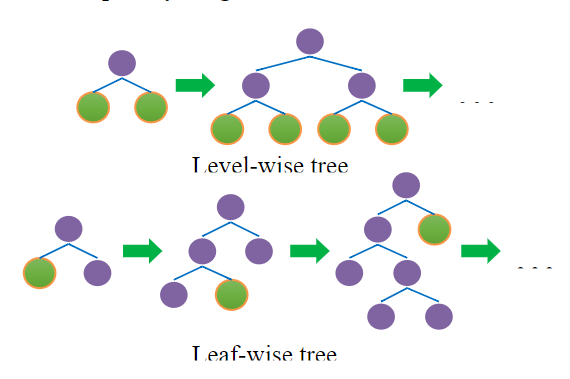
\includegraphics[width=\linewidth]{LGBM.png}}
    \caption{Light Gradient Boosting Machine (LGBM)}
    \label{lgbm}
\end{figure}

Algoritma LightGBM dikembangkan oleh Microsoft yang memberikan kemampuan yang efisien dari algoritma \textit{Gradient Boosting}. LightGBM memiliki 
karakteristik yang membedakannya dengan algoritma \textit{tree boosting} lainnya adalah dengan membelah pohon secara memanjang 
(\textit{leaf-wise tree growth}) dengan yang paling cocok, sedangkan algoritma \textit{tree boosting} lainnya membagi pohon secara mendalam atau sejajar (\textit{level-wise tree growth}) 
yang ditunjukkan pada ``Fig. ~\ref{lgbm}'' \cite{b30}.

LightGBM menggunakan dua teknik utama, yaitu \textit{Exclusive Feature Bundling} (EFB) dan \textit{Gradient-based One-Side Sampling} (GOSS), untuk meningkatkan kecepatan dan 
mengurangi penggunaan memori. EFB menggabungkan fitur-fitur yang jarang digunakan menjadi satu fitur, mengurangi jumlah fitur yang perlu diproses. GOSS, 
di sisi lain, memilih sampel dengan gradien besar dan mempertahankan distribusi data, sehingga mengurangi jumlah data yang diproses tanpa kehilangan akurasi. 
Proses pelatihan LightGBM dimulai dengan membangun pohon keputusan dari data pelatihan, dan setiap iterasi bertujuan untuk mengurangi kesalahan dari model sebelumnya 
dengan menggunakan gradien untuk mengarahkan perbaikan \cite{b31}.

\subsection{Ensemble (Stacking)}

\textit{Stacking} termasuk dalam kategori \textit{ensemble learning} yang didalamnya terdapat proses tumpukan dari beberapa algoritma klasifikasi tunggal. Dalam penggunaannya, terdapat dua level 
model pembelajaran yang akan digunakan ketika metode \textit{stacking} diterapkan, yang pertama adalah model pembelajaran level-0 yang di kenal sebagai \textit{base learner}, dan model 
pembelajaran level-1 yang merupakan \textit{meta-learner}. Model \textit{Stacking} ini menggunakan model XGBoost, LightGBM, dan CatBoost sebagai \textit{base learner}, dan LR sebagai \textit{meta learner} \cite{b32}. 
Ilustrasi dari proses \textit{stacking} digambarkan melalui ``Fig. ~\ref{stacking}''.

\begin{figure}[htbp]
    \centerline{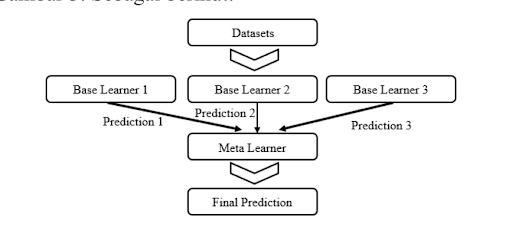
\includegraphics[width=\linewidth]{stacking.png}}
    \caption{Ensemble dengan Stacking}
    \label{stacking}
\end{figure}

\section{Dataset}

\subsection{Spaceship Dataset}
Dataset Spaceship Titanic adalah kumpulan data yang memuat informasi tentang penumpang kapal luar angkasa dan keterkaitannya dengan keputusan mereka untuk diangkut ke dimensi lain atau tidak. 
Tujuan dari dataset ini adalah untuk memprediksi apakah seorang penumpang akan diangkut ke dimensi lain atau tidak.

Dataset ini menyediakan fitur-fitur untuk melakukan prediksi. \textit{HomePlanet} adalah planet asal penumpang, \textit{CryoSleep} menunjukkan apakah penumpang akan dibekukan atau tidak, 
VIP menunjukkan apakah penumpang memiliki layanan VIP atau tidak, \textit{RoomService, FoodCourt, shopping mall, Spa, VRDeck} adalah fitur-fitur yang menunjukkan pengeluaran penumpang, 
\textit{Transported} adalah target class yang menunjukkan apakah penumpang diangkut ke dimensi lain atau tidak.

Dalam dataset ini, fitur-fitur yang digunakan untuk prediksi meliputi \textit{HomePlanet}, \textit{CryoSleep}, VIP, \textit{RoomService, FoodCourt, shopping mall, Spa, VRDeck}, dan \textit{Transported}. Fitur-fitur ini 
digunakan untuk memprediksi apakah seorang penumpang akan diangkut ke dimensi lain atau tidak. 

Dalam penelitian ini, dataset Spaceship Titanic digunakan untuk memprediksi apakah seorang penumpang akan diangkut ke dimensi lain atau tidak. Dataset ini digunakan untuk mempelajari 
pola dan hubungan antara fitur-fitur yang digunakan untuk prediksi. Dengan menggunakan dataset ini, penelitian ini dapat membantu dalam meningkatkan akurasi prediksi dan meningkatkan 
kemampuan sistem dalam memprediksi keputusan penumpang.

\subsection{Bank Churn Dataset}
Dataset Bank Churn adalah kumpulan data yang memuat informasi tentang nasabah bank dan keterkaitannya dengan keputusan mereka untuk berhenti menggunakan layanan atau produk yang ditawarkan oleh bank tersebut. 
Tujuan dari dataset ini adalah untuk memprediksi apakah seorang nasabah akan tetap menggunakan akun mereka atau akan menutupnya.

Dataset ini menyediakan fitur-fitur untuk melakukan prediksi. \textit{Id} dan \textit{customerId} adalah dua fitur yang digunakan sebagai identitas dari \textit{customer} yang sifatnya unik. \textit{Surname} adalah nama keluarga dari nasabah, 
\textit{CreditScore} adalah skor kredit dari nasabah, \textit{Geography} menunjukkan geografi, \textit{Gender} menunjukkan jenis kelamin, \textit{Age} menunjukkan umur, \textit{Tenure} menunjukkan waktu nasabah telah memiliki akun, \textit{Balance} adalah jumlah 
uang tersimpan dalam akun nasabah, \textit{NumOfProducts} mengacu pada jumlah produk atau layanan perbankan yang dimiliki oleh seorang nasabah, \textit{isActiveMember} mengacu pada status keanggotaan aktif, dan \textit{Estimated Salary} 
adalah gaji estimasi dari nasabah.

Dalam dataset ini, target kelas yang digunakan adalah \textit{'Exited'}. Pada data \textit{training}, kelas ini memiliki nilai biner, yaitu 1 dan 0 seperti pada ``Fig. ~\ref{churn_distribution}''. Prediksi akan dilakukan terhadap kelas ini dan kalkulasi yang dilakukan adalah 
mencari probabilitas dari seorang nasabah akan menutup akun menggunakan nilai kontinu. Semakin tinggi nilai nya, maka semakin tinggi kemungkinan orang tersebut akan menutup akun, berlaku sebaliknya untuk nilai 
probabilitas yang semakin rendah. Melalui data latih, dataset menunjukkan persentase dominan terhadap \textit{Not Exited}. Melalui \textit{heatmap} korelasi fitur kontinu ``Fig. ~\ref{churn_corr}'', tidak ada fitur yang memiliki korelasi yang tinggi. 
Berdasarkan pengamatan pada \textit{heatmap} ``Fig. ~\ref{churn_nan}'', tidak ada \textit{missing value} ditemukan pada data latih maupun data uji.

\begin{figure}[htbp]
    \centerline{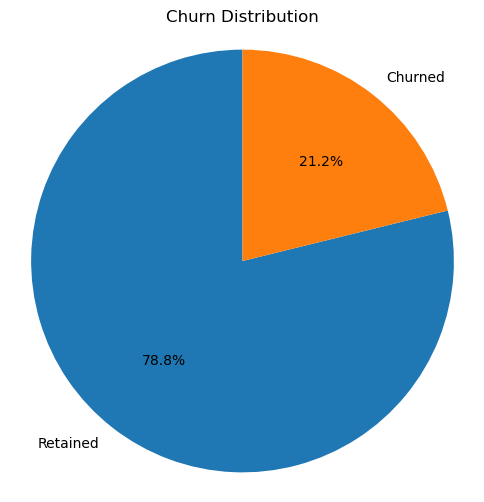
\includegraphics[width=\linewidth, scale=0.7]{churn_distribution.png}}
    \caption{Distribusi kelas Bank Churn}
    \label{churn_distribution}
\end{figure}

\begin{figure}[htbp]
    \centerline{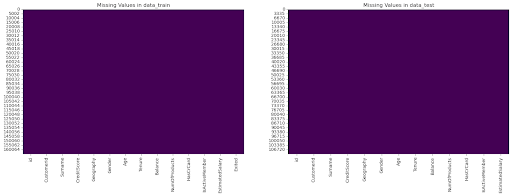
\includegraphics[width=\linewidth]{churn_nan.png}}
    \caption{Nilai NaN Dataset Bank Churn}
    \label{churn_nan}
\end{figure}

\begin{figure}[htbp]
    \centerline{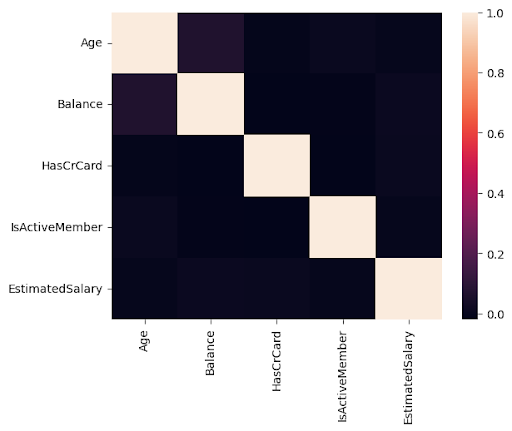
\includegraphics[width=\linewidth, scale=0.5]{churn_corr_heatmap.png}}
    \caption{Heatmap Fitur Dataset Bank Churn}
    \label{churn_corr}
\end{figure}

\subsection{Horse Health Dataset}
Dataset Predict Health Outcomes of Horses adalah kumpulan data yang memuat informasi tentang kondisi kesehatan kuda dan keterkaitannya 
dengan hasil akhir kesehatan mereka, seperti apakah mereka akan sembuh, mati, atau di-euthanasia. Tujuan dari dataset ini adalah untuk 
memprediksi hasil kesehatan kuda berdasarkan berbagai fitur medis yang tersedia.

Fitur-fitur dataset:
\begin{itemize}
    \item 'surgery': Apakah kuda tersebut menjalani operasi (yes/no)
    \item 'age': Usia kuda (adult)
    \item 'hospital number': Nomor rumah sakit tempat kuda dirawat
    \item 'rectal temp': Suhu rektal kuda dalam derajat Celcius
    \item 'pulse': Denyut nadi kuda per menit 
    \item 'respiratory rate': Laju pernapasan kuda per menit 
    \item 'temp of extremities': Suhu ekstrimitas ('cool'/'normal'/'code')
    \item 'peripheral pulse': Denyut nadi perifer ('normal'/'reduced')
    \item 'mucous membrane': Warna membran mukosa ('pale pink'/'normal pink'/'dark cyanotic')
    \item 'capillary refill time': Waktu pengisian kembali kapiler ('less 3 sec'/'more 3 sec')
    \item 'pain': Tingkat rasa sakit ('alert'/'depressed'/'mild pain'/'severe pain'/extreme pain')
    \item 'peristalsis': Gerakan peristaltik usus ('normal'/'hypomotile'/'hypermotile'/'absent')
    \item 'abdominal distention': Distensi abdominal (slight/moderate/none)
    \item 'nasogastric tube': Kehadiran selang nasogastrik (yes/no)
    \item 'nasogastric reflux': Refluks nasogastrik (yes/no)
    \item 'nasogastric reflux pH': pH refluks nasogastrik
    \item 'rectal exam feces': Hasil pemeriksaan rektal (normal/decreased)
    \item 'abdomen': Kondisi perut (normal/firm/distend small/distend large)
    \item 'packed cell volume': Volume sel darah terpak (dalam persen)
    \item 'total protein': Total protein dalam darah (dalam g/dL)
    \item 'abdomo appearance': Penampakan cairan perut (serosanguious/cloudy)
    \item 'abdomo protein': Protein dalam cairan perut (dalam g/dL)
    \item 'surgical lession': Protein dalam cairan perut (dalam g/dL)
    \item 'lession 1', 'lession 2', 'lession 3': Identifikasi lesi (numerik)
    \item 'cp data': Data terkair CP (yes/no)
    \item 'outcome': Hasil akhir kesehatan kuda (lived/died/euthanized)
\end{itemize}

Statistik dan distribusi fitur dataset Horse Health:
\begin{itemize}
    \item Fitur kategorikal seperti \textit{surgery, age, temp of extremities, peripheral pulse, mucousmembrane, capillary refill time, pain, peristalsis, abdominaldistention, nasogastrictube, nasogastricreflux, rectalexamfeces, abdomen, abdomo appearance, surgical lesion, cp data}, dan \textit{outcome} dikodekan menggunakan LabelEncoder.
    \item Fitur numerik meliputi \textit{hospital number, rectal temp, pulse, respiratory rate, nasogastric reflux pH, packed cell volume, total protein, abdomo protein, lesion 1, lesion 2}, dan \textit{lesion 3}.
\end{itemize}

\begin{figure}[htbp]
    \centerline{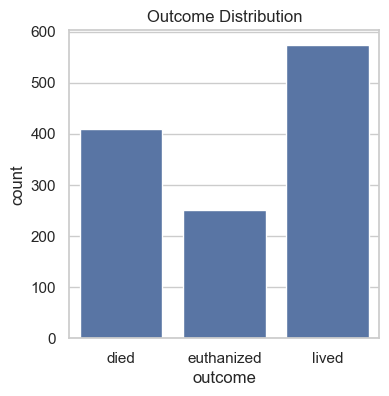
\includegraphics[width=\linewidth, scale=0.5]{horse_distribution.png}}
    \caption{Distribusi Outcome Dataset Horse Health}
    \label{horse_distribution}
\end{figure}

\begin{figure}[htbp]
    \centerline{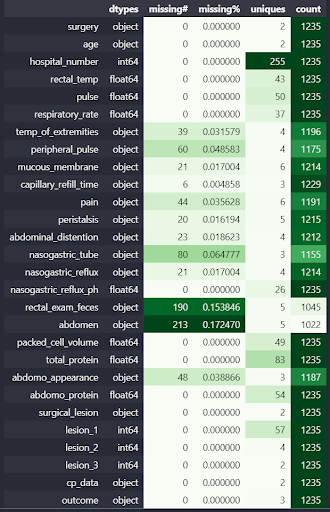
\includegraphics[width=\linewidth, scale=0.5]{horse_feature_description.png}}
    \caption{Statistik Deskriptif Dataset Horse Health}
    \label{horse_description}
\end{figure}

\begin{figure}[htbp]
    \centerline{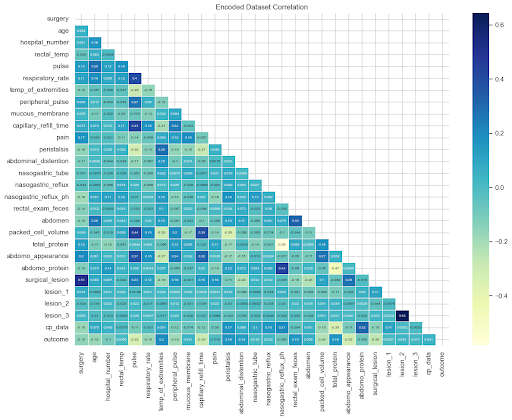
\includegraphics[width=\linewidth, scale=0.5]{horse_corr.png}}
    \caption{Korelasi Fitur Dataset Horse Health}
    \label{horse_corr}
\end{figure}

Dataset ini menunjukkan distribusi hasil kesehatan kuda sebagai berikut: \textit{lived} (kuda yang bertahan hidup), \textit{died} (kuda yang meninggal), dan \textit{euthanized} (kuda yang di-euthanasia). 
Grafik distribusi hasil kesehatan ``Fig. ~\ref{horse_distribution}'' menunjukkan bahwa sebagian besar kuda dalam dataset ini bertahan hidup, dengan proporsi yang lebih kecil meninggal atau di-euthanasia. 
Analisis korelasi antar fitur ``Fig. ~\ref{horse_corr}'' dalam dataset ini menunjukkan hubungan antara berbagai fitur dan hasil kesehatan. Heatmap korelasi menunjukkan bahwa beberapa fitur memiliki korelasi 
yang lebih tinggi dengan hasil kesehatan kuda, yang dapat digunakan untuk membangun model prediktif yang lebih akurat.

\subsection{Keep-it-Dry Dataset}

Dataset Keep-it-Dry merepresentasikan hasil dari product testing untuk produk absorben berdasarkan hasil pengukuran dan uji laboratorium tertentu. Setiap produk absorben yang diujikan memiliki 
\textit{‘product code’} dengan empat buah atribut tetap (\textit{fixated attributes}), yang disimpan pada fitur \textit{‘attribute 0’} hingga \textit{‘attribute 3’}. Tiap \textit{record} pada dataset ini juga memiliki fitur \textit{'loading'}, yang 
menyatakan banyaknya cairan yang berhasil diserap untuk produk absorben yang diujikan. Hasil pengukuran untuk tiap pengujian berbeda juga tersedia dan direpresentasikan dalam fitur \textit{‘measurement 0’} 
hingga \textit{‘measurement 17’}. Kelas target dalam dataset ini adalah \textit{'failure'} dengan nilai biner 0 dan 1, yang menyatakan apakah produk tersebut lolos ataupun gagal.

\textit{Training set} pada dataset ini memiliki 26,570 \textit{records} dengan 20,775 \textit{records} untuk proses \textit{submission} dengan kelas \textit{'failure'}=0 menjadi \textit{majority class} ``Fig. ~\ref{kid_distribution}''. Dari 25 fitur yang tersedia, terdapat 3 fitur yang memiliki tipe data \textit{object}: 
\textit{‘product code’, ‘attribute 0’}  dan \textit{‘attribute 1’}. Melalui peta persebaran nilai NaN ``Fig. ~\ref{kid_nan}'', terdapat 9 fitur tanpa nilai NaN: \textit{‘id’, ‘product code’, ‘loading’, ‘attribute 0’} hingga ‘attribute 3’, serta \textit{‘measurement 0’} hingga \textit{‘measurement 2’}. 
Melalui \textit{heatmap} korelasi fitur kontinu ``Fig. ~\ref{kid_corr}'', tidak ditemukan adanya fitur dengan korelasi linear yang tinggi.

\begin{figure}[htbp]
    \centerline{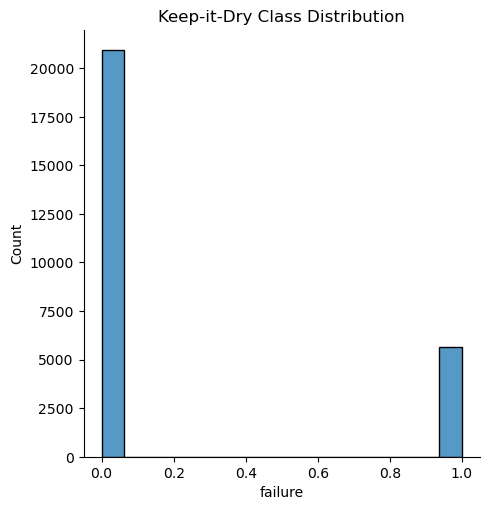
\includegraphics[width=\linewidth, scale=0.5]{KID_Class_Distribution.png}}
    \caption{Distribusi Kelas Dataset Keep-it-Dry}
    \label{kid_distribution}
\end{figure}

\begin{figure}[htbp]
    \centerline{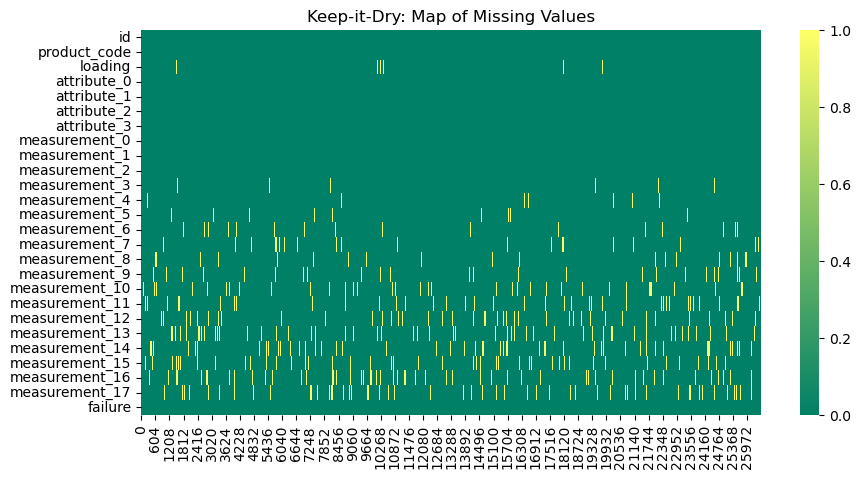
\includegraphics[width=\linewidth, scale=0.5]{KID_Missing_Values.png}}
    \caption{Distribusi nilai NaN Dataset Keep-it-Dry}
    \label{kid_nan}
\end{figure}

\begin{figure}[htbp]
    \centerline{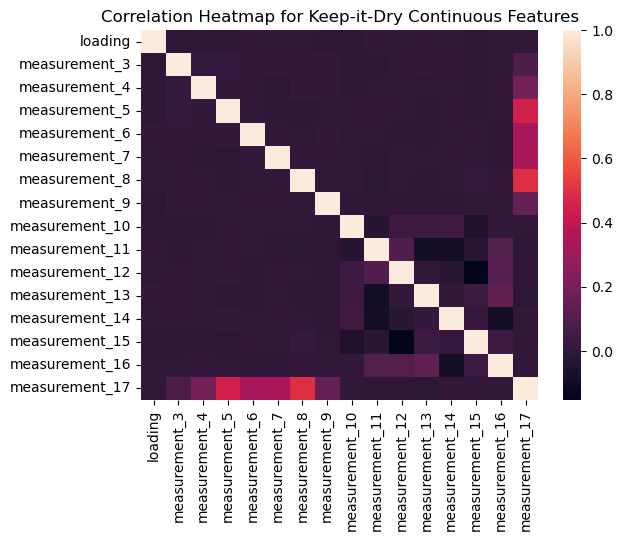
\includegraphics[width=\linewidth, scale=0.5]{KID_Continuous_Features_Correlation_Heatmap.png}}
    \caption{Korelasi Fitur Dataset Keep-it-Dry}
    \label{kid_corr}
\end{figure}

\section{Metodologi}

\subsection{Imputasi Data}
Imputasi data adalah proses mengganti nilai yang hilang dalam dataset dengan nilai yang diperkirakan berdasarkan informasi yang tersedia. 
Kehilangan data dapat disebabkan oleh berbagai alasan seperti kesalahan pengukuran, pengabaian, atau masalah teknis. Nilai yang hilang dalam dataset bisa mengurangi 
kualitas analisis dan menyebabkan model \textit{machine learning} menjadi bias jika tidak ditangani dengan benar \cite{b35}. Oleh karena itu, imputasi merupakan 
langkah penting dalam data preprocessing untuk memastikan bahwa dataset yang digunakan dalam analisis atau pelatihan model adalah representatif dan lengkap.

Dalam penelitian ini, beberapa teknik imputasi data yang digunakan adalah sebagai berikut.

\begin{itemize}
    \item \textit{Mean Imputation} \\
    Mengganti nilai yang hilang dengan rata-rata nilai dalam kolom tersebut. Teknik ini sederhana dan sering digunakan, terutama jika data 
    memiliki distribusi normal. Namun, \textit{mean imputation} bisa memperkecil variasi data dan mengabaikan korelasi antar variabel.
    \item \textit{Median Imputation} \\
    Mengganti nilai yang hilang dengan nilai tengah dalam kolom tersebut. Opsi ini lebih tahan terhadap \textit{outlier} dibandingkan \textit{mean imputation}, 
    sehingga lebih baik digunakan jika data memiliki distribusi yang \textit{skewed}. \textit{Median imputation} juga mempertahankan distribusi data lebih baik daripada \textit{mean imputation}.
    \item \textit{Mode Imputation} \\
    Mengganti nilai yang hilang dengan nilai yang paling sering muncul dalam kolom tersebut. Cocok untuk data kategori, karena menggantikan nilai yang hilang 
    dengan kategori yang paling umum. \textit{Mode imputation} dapat mempertahankan distribusi kategori dalam data, tetapi mungkin tidak ideal untuk data numerik.
    \item \textit{K-Nearest Neighbors Imputation (KNN Imputation)} \\
    Menggunakan nilai-nilai dari data yang paling mirip untuk memperkirakan nilai yang hilang. KNN \textit{imputation} mempertimbangkan kedekatan atau kemiripan antara sampel, 
    sehingga dapat menghasilkan imputasi yang lebih akurat dibandingkan metode sederhana seperti mean atau median. Namun, KNN \textit{imputation} bisa jadi komputasi intensif, terutama 
    untuk dataset yang besar.
    \item \textit{Multiple Imputation}
    Menghasilkan beberapa set nilai yang hilang untuk mencerminkan ketidakpastian yang lebih baik dalam imputasi. Teknik ini menciptakan beberapa dataset lengkap, menganalisis masing-masing, 
    dan menggabungkan hasilnya untuk memberikan estimasi yang lebih akurat dan tidak bias. \textit{Multiple imputation} menangani ketidakpastian dalam data yang hilang dengan lebih baik dibandingkan metode imputasi tunggal.

\end{itemize}

\subsection{Data Encoding}
\textit{Data encoding} adalah proses mengubah data kategori menjadi bentuk numerik agar dapat diproses oleh algoritma \textit{machine learning} yang umumnya hanya dapat bekerja dengan data numerik \cite{b36}. 
Data kategori, seperti jenis kelamin atau status perkawinan, perlu diubah menjadi format yang dapat dipahami oleh model matematis. Tanpa \textit{encoding}, algoritma \textit{machine learning} tidak dapat 
menggunakan informasi dari fitur kategori, karena mereka mengharapkan input dalam bentuk numerik. \textit{Encoding} sangat penting untuk memastikan bahwa model dapat memahami dan memanfaatkan 
data kategori dengan benar.

Dalam penelitian ini, beberapa teknik \textit{encoding} yang digunakan adalah sebagai berikut.

\begin{itemize}
    \item \textit{Label Encoding}: memberikan label numerik untuk setiap kategori dalam fitur. Digunakan saat kategori memiliki urutan tertentu (ordinal).
    Meskipun sederhana, label encoding dapat menimbulkan masalah jika kategori tidak memiliki hubungan ordinal, karena model mungkin akan menafsirkan urutan numerik sebagai representasi hubungan ordinal.
    \item \textit{One-Hot Encoding}: membuat kolom biner terpisah untuk setiap kategori unik dalam fitur. Menghindari memberikan urutan yang tidak diinginkan pada data kategori. 
    \textit{One-hot encoding} sangat efektif untuk menghindari masalah yang ditimbulkan oleh \textit{label encoding} pada data non-ordinal. Namun, metode ini dapat menyebabkan peningkatan dimensi data yang signifikan jika jumlah kategori banyak.
    \item \textit{Ordinal Encoding}: mengurutkan kategori dalam fitur dan memberikan nilai numerik berdasarkan urutan tersebut. Cocok untuk data ordinal dimana ada urutan yang jelas di antara kategori, seperti \textit{rating} (buruk, cukup, baik, sangat baik). 
    \item \textit{Binary Encoding}: kombinasi dari \textit{label encoding} dan \textit{one-hot encoding} yang menghasilkan representasi biner. Teknik ini mengurangi dimensi data dibandingkan dengan \textit{one-hot encoding} dan masih memberikan representasi yang baik untuk data kategori.
\end{itemize}

\subsection{Data Scaling}
\textit{Data scaling} adalah proses menormalkan atau mengubah skala data agar semua fitur berada dalam rentang yang sama, biasanya 0 hingga 1 atau -1 hingga 1. Hal ini penting agar algoritma \textit{machine learning} tidak bias 
terhadap fitur dengan skala yang lebih besar \cite{b37}. Misalnya, fitur yang diukur dalam ribuan unit dapat mendominasi fitur lain yang diukur dalam skala yang lebih kecil, sehingga mempengaruhi kinerja model. 
\textit{Data scaling} membantu dalam mempercepat konvergensi model selama pelatihan dan meningkatkan performa prediksi.

Dalam penelitian ini, beberapa teknik \textit{data scaling} yang digunakan adalah sebagai berikut.

\begin{itemize}
    \item \textit{Standard Scaler}: adalah menormalkan data sehingga memiliki mean 0 dan standar deviasi 1. Cocok untuk data yang mendekati distribusi normal. 
    Dengan \textit{Standard Scaler}, kita memastikan bahwa setiap fitur memiliki kontribusi yang seimbang dalam model. \textit{Standard Scaler} menjaga hubungan linear antara fitur 
    dan memungkinkan model untuk lebih efektif mempelajari pola dalam data.
    \item \textit{MinMax Scaler}: adalah mengubah skala data sehingga berada dalam rentang antara 0 dan 1. Cocok untuk data yang tidak memiliki \textit{outlier} ekstrem. 
    \textit{MinMax Scaler} mempertahankan hubungan proporsional antara nilai asli dan nilai skala.
    \item \textit{Robust Scaler}: mengurangi pengaruh \textit{outlier} dengan menggunakan median dan \textit{interquartile range}. 
    Cocok untuk data dengan \textit{outlier} yang signifikan. \textit{Robust Scaler} memastikan bahwa \textit{scaling} tidak dipengaruhi oleh nilai ekstrim 
    yang dapat mendistorsi distribusi data. \textit{Robust Scaler} menjaga robustness model terhadap \textit{outlier}.
\end{itemize}

\subsection{Imbalance Handling}

\textit{Imbalance handling} adalah proses mengatasi ketidakseimbangan kelas dalam dataset, dimana jumlah sampel pada satu kelas jauh lebih banyak 
dibandingkan kelas lainnya. Ketidakseimbangan ini dapat menyebabkan model \textit{machine learning} bias terhadap kelas mayoritas dan mengabaikan kelas minoritas \cite{b38}, 
sehingga menghasilkan prediksi yang tidak akurat. Ketidakseimbangan kelas dapat mengurangi kemampuan model untuk mendeteksi kelas minoritas yang penting. Opsi yang tersedia untuk 
\textit{imbalance handling} yang digunakan pada penelitian ini adalah sebagai berikut.

\begin{itemize}
    \item \textit{Oversampling}: menambah jumlah sampel dari kelas minoritas. Teknik ini termasuk ROS (\textit{Random Over Sampler}) maupun teknik seperti SMOTE (\textit{Synthetic Minority Over-sampling Technique}), 
    yang menciptakan sampel baru dari kelas minoritas dengan menginterpolasi antara sampel yang ada. 
    \textit{Oversampling} dapat meningkatkan representasi kelas minoritas dalam dataset. Namun, \textit{oversampling} dapat menyebabkan 
    \textit{overfitting} jika sampel yang baru diciptakan terlalu mirip dengan yang sudah ada.
    \item \textit{Undersampling}: mengurangi jumlah sampel dari kelas mayoritas, seperti dengan menggunakan RUS (\textit{Random Under Sampler}). 
    Teknik ini menghapus sebagian sampel dari kelas mayoritas untuk mencapai keseimbangan. Meskipun dapat membantu mengatasi ketidakseimbangan, 
    \textit{undersampling} berisiko menghilangkan informasi penting dari kelas mayoritas. \textit{Undersampling} membantu dalam mengurangi ukuran dataset dan mempercepat 
    proses pelatihan.
    \item \textit{Hybrid Methods}: menggabungkan \textit{oversampling} dan \textit{undersampling} untuk mendapatkan keseimbangan yang lebih baik. 
    \textit{Hybrid methods} memanfaatkan kelebihan dari kedua pendekatan untuk menciptakan dataset yang lebih seimbang. \textit{Hybrid methods} dapat 
    mengurangi risiko overfitting dan underfitting yang mungkin terjadi pada \textit{oversampling} atau \textit{undersampling} tunggal.
\end{itemize}

\subsection{Principal Component Analysis (PCA)}

\textit{Principal Component Analysis} (PCA) adalah teknik pengurangan dimensi yang mengubah data ke dalam set baru dari variabel (\textit{principal components}) yang mempertahankan 
variabilitas maksimum dalam data. PCA membantu dalam mengurangi jumlah fitur dan mengatasi masalah multikolinearitas. Dalam PCA, data diubah menjadi 
komponen utama yang merupakan kombinasi linear dari fitur asli dengan varian terbesar. Komponen utama ini mempertahankan 
sebanyak mungkin informasi dari data asli. PCA mengidentifikasi arah variabilitas maksimum dalam data dan mentransformasikannya menjadi 
set baru dari fitur yang tidak berkorelasi.

Tujuan dari PCA adalah mengurangi jumlah fitur dalam dataset, mengatasi masalah multikolinearitas, meningkatkan efisiensi komputasi, dan meningkatkan performa model 
\textit{machine learning} \cite{b39}. Dengan mengurangi dimensi data, PCA membantu dalam visualisasi data, mempercepat waktu pelatihan model, dan mengurangi risiko \textit{overfitting}. 
PCA juga membantu dalam mengidentifikasi fitur yang paling penting dan mengabaikan \textit{noise} dalam data. Transformasi data menggunakan PCA memungkinkan model untuk fokus pada 
komponen yang paling signifikan dan mengurangi beban komputasi.

\subsection{Optimalisasi Hyperparameter: GridSearchCV}

Akurasi dari suatu model dapat ditingkatkan dengan memanfaatkan GridSearchCV \cite{b40}.  GridSearchCV adalah sebuah kelas yang disediakan oleh \textit{framework} scikit-learning. 
Tujuan dari GridSearchCV adalah untuk menentukan kombinasi \textit{hyperparameter} yang menghasilkan nilai terbaik \cite{b41}. Grid search bekerja dengan cara melakukan seleksi terhadap model 
dan \textit{hyperparameter} terbaik. Untuk memperoleh model dan \textit{hyperparameter} terbaik, teknik ini akan melakukan pengujian terhadap 
seluruh kombinasi \textit{hyperparameter} dari \textit{dictionary} yang telah didefinisikan. Untuk setiap kombinasi yang berhasil dibangkitkan, akan dilakukan 
validasi terhadap model klasifikasi dengan menggunakan \textit{k-fold  cross-validation} (CV). Setiap \textit{k-fold cross-validation} dari model akan 
menghasilkan evaluation index yang akan menjadi acuan dalam menentukan model klasifikasi terbaik \cite{b42}.

\begin{equation}
    \text{E} = \frac{1}{K} \sum_{k=1}^{K} E_k \label{gridsearch_eq}
\end{equation}

Setiap tahapan \textit{K-fold cross-validation} dilakukan dengan melakukan repetisi sebanyak K kali pada data yang terbagi menjadi K bagian. Pada setiap perulangan 1/k dataset 
digunakan sebagai data uji dan sisanya akan bertindak sebagai data latih \cite{b43}. \textit{K-fold cross-validation} akan menghitung rata-rata dari kalkulasi yang telah dilakukan dan menjadikannya sebagai 
index performansi dari model klasifikasi. Setelah itu, parameter klasifikasi diubah ke kombinasi lainnya dan proses validasi dilakukan kembali. Tahapan ini akan terus berlanjut dan setiap iterasi akan menghasilkan 
akurasi model. Persamaan dari \textit{K-fold cross-validation} dapat dilihat pada ``\eqref{gridsearch_eq}''. Diagram alir dari proses GridSearchCV dapat dilihat pada ``Fig. ~\ref{gridsearch_flow}''.

\begin{figure}[htbp]
    \centerline{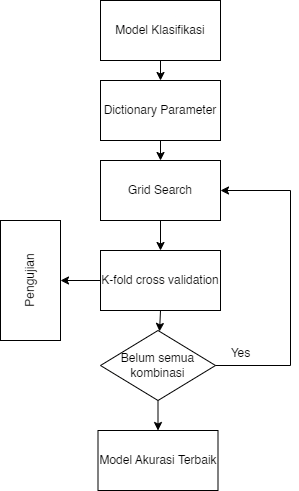
\includegraphics[scale=0.5]{gridsearch.png}}
    \caption{Diagram Alir GridSearchCV}
    \label{gridsearch_flow}
\end{figure}

\subsection{Optimalisasi Hyperparameter: Optuna}

Optuna adalah sebuah pustaka yang melakukan optimasi terhadap \textit{hyperparameter tuning}. 
Untuk menemukan \textit{hyperparameter} terbaik terkadang, melakukan proses training dan evaluasi secara repetitif hanya akan
membuang waktu dan tenaga \cite{b44}. Oleh karena itu, Optuna berperan untuk melakukan automasi terhadap optimasi \textit{hyperparameter}.

Optuna menggunakan landasan utama seperti fungsi objektif yang digunakan sebagai penentu metrik yang ingin dioptimalkan, 
ruang pencarian yang mendefinisikan rentang valid atau kumpulan nilai diskrit dari setiap parameter, trial yang mengevaluasi 
fungsi objektif dengan \textit{hyperparameter} tertentu, dan sampler yang menentukan parameter baru yang digunakan.

Langkah-langkah Optuna dalam memilih \textit{hyperparameter} yang optimal terdiri dari: Penentuan fungsi objektif, 
pemilihan sampler, Iterasi dan Optimasi \cite{b45}. Prosedur dasar Optuna dapat dilihat pada ``Fig. ~\ref{optuna_flow}''.

\begin{figure}[htbp]
    \centerline{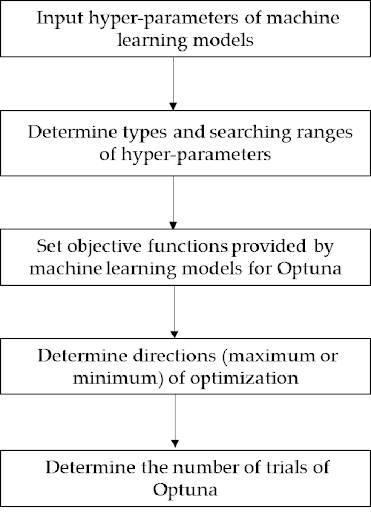
\includegraphics[scale=0.5]{optuna.png}}
    \caption{Diagram Alir Optuna}
    \label{optuna_flow}
\end{figure}

\subsection{Evaluasi Model}

Pada pengujian yang dilakukan di artikel ini, evaluasi model dilakukan dengan menggunakan metode tabulasi silang (\textit{Confusion Matrix}). 
Proses evaluasi ini adalah dengan menyusun matriks yang berisi kelas data asli pada barisnya dan kelas data hasil prediksi pada kolomnya \cite{b46}. 
Ilustrasi \textit{Confusion Matrix} dapat dilihat pada ``Fig. ~\ref{confusionmatrix}''.

\begin{figure}[htbp]
    \centerline{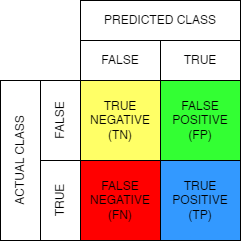
\includegraphics[scale=0.5]{confusionmatrix.png}}
    \caption{Confusion Matrix}
    \label{confusionmatrix}
\end{figure}

Pada ``Fig. ~\ref{confusionmatrix}'', terdapat 4 lokasi grid dengan kondisi yang berbeda. \textit{True Negative} menandakan jumlah prediksi 
negatif yang berhasil diprediksi secara benar. \textit{False Positive} menandakan jumlah \textit{actual negative} yang salah diprediksi sebagai positif. 
\textit{False Negative} menandakan jumlah \textit{actual positive} yang salah diprediksi sebagai \textit{negative} \cite{b47}.

Selain itu, digunakan beberapa metode \textit{scoring} sebagai berikut.

\begin{itemize}
    \item \textbf{Recall} \\
    \textit{Recall} (perolehan) berhubungan dengan kemampuan suatu sistem temu balik dalam menemukan dokumen yang relevan. 
    Hal ini berarti perolehan (\textit{recall}) adalah bagian dari proses temu balik informasi yang dapat digunakan sebagai alat ukur tingkat efektivitas suatu sistem temu balik informasi \cite{b48}. 
    Rumus \textit{Recall} dapat dilihat pada ``\eqref{recall}''. 
    \item \textbf{Precision} \\
    \textit{Precision} adalah jumlah kelompok dokumen relevan dari total jumlah dokumen yang ditemukan oleh sistem. 
    Berdasarkan penjelasan tersebut, rumus \textit{precision} dapat dilihat pada ``\eqref{precision}''.
    \item \textbf{Accuracy} \\
    \textit{Accuracy} adalah kedekatan antara nilai prediksi dengan nilai aktual. Dalam memilih \textit{accuracy}, 
    seluruh komponen terlibat. Rumus \textit{accuracy} dapat dilihat pada ``\eqref{accuracy}''.
    \item F-Measure (F1-Score) \\
    Metrik ini menggabungkan precision dan recall, memberikan gambaran menyeluruh tentang kemampuan model dalam 
    mengidentifikasi contoh positif secara akurat dan meminimalkan false positive. Rumus F-Measure dapat dilihat 
    pada ``\eqref{f1}''.
    \item \textbf{AUC-ROC} \\
    AUC-ROC adalah metrik evaluasi yang mengukur kemampuan model klasifikasi dalam membedakan antara kelas positif dan negatif. Metrik ini dihitung dengan 
    menghitung luas area di bawah kurva ROC (\textit{Receiver Operating Characteristic}). Kurva ROC diplotkan dengan \textit{True Positive Rate} (TPR) pada sumbu-y dan 
    \textit{False Positive Rate} (FPR) pada sumbu-x. AUC = 1.0 berarti Performa model sempurna, semua contoh positif diidentifikasi dengan benar tanpa false positive. 
    AUC = 0.5 berarti performa model tidak lebih baik dari menebak secara acak. Nilai antara 0.5 dan 1.0 berarti menunjukkan performa model di antara acak dan sempurna \cite{b48}.
    
    AUC tidak memberikan informasi tentang presisi dan recall secara langsung, sehingga perlu dipertimbangkan metrik lain untuk mengukur performa model 
    secara komprehensif. AUC dapat sensitif terhadap outlier dalam data, sehingga perlu dilakukan outlier detection sebelum menghitung AUC \cite{b49}.

    \item \textbf{Cross-Validation (CV)} \\
    \textit{Cross-Validation} (CV) adalah teknik evaluasi model yang membagi data menjadi beberapa subset (fold) dan melatih model beberapa kali dengan menggunakan subset yang berbeda sebagai data 
    latih dan data uji. Tujuannya adalah untuk mendapatkan perkiraan performa model yang lebih akurat dan stabil. \textit{K-fold Cross-Validation} membagi data menjadi k subset, dan model dilatih 
    k kali dengan menggunakan k-1 subset sebagai data latih dan 1 subset sebagai data uji. \textit{Leave-one-out Cross-Validation} membagi data menjadi n subset, di mana n adalah jumlah data. 
    Model dilatih n kali dengan menggunakan n-1 subset sebagai data latih dan 1 data sebagai data uji. \textit{Stratified Cross-Validation} membagi data menjadi subset berdasarkan kelasnya, 
    dan CV dilakukan dengan memastikan proporsi kelas pada data latih dan data uji sama dengan proporsi kelas pada data keseluruhan. \cite{b50}. 
    CV memiliki kelebihan dapat digunakan untuk memperkirakan performa model yang lebih akurat dan stabil, memilih model terbaik, serta membantu dalam proses pemilihan 
    parameter terbaik. Kekurangan dari CV adalah waktu komputasi yang cukup lama.
\end{itemize}

\begin{equation}
    Recall = \frac{TP}{TP+FN} \label{recall}
\end{equation}

\begin{equation}
    Precision = \frac{TP}{TP+FP} \label{precision}
\end{equation}

\begin{equation}
    Accuracy = \frac{TP + TN}{TP+FP+TN+FN} \label{accuracy}
\end{equation}

\begin{equation}
    F1 = 2.\frac{ Precision * Recall}{Precision \times Recall} \label{f1}
\end{equation}

\section{Hasil dan Diskusi}
\subsection{Dataset Spaceship}

Pada tahap pemrosesan awal, yang dilakukan adalah menghapus kolom yang tidak relevan untuk mengurangi kompleksitas data, kemudian melakukan one-hot encoding 
dan label encoding pada kolom kategorikal. Kolom boolean diubah menjadi tipe data integer untuk memastikan konsistensi format data. Selanjutnya, melakukan normalisasi Z-Score pada variabel 
kontinu untuk menstandarkan data sehingga setiap fitur memiliki mean nol dan standar deviasi satu, memastikan tidak ada fitur yang mendominasi karena skala yang berbeda. Scaling data dilakukan dengan menggunakan 
Standard Scaling (ST). dari tahapan tersebut terbentuk 2 clean dataset dengan teknik pemrosesan awal yang yang akan diujikan pada tahap dataset selection untuk masing masing model.

Pada percobaan menggunakan model klasifikasi KNN, diperoleh akurasi sebesar 0.52 dengan menggunakan PCA (Component Analysis) dan k=3. Namun ketika menambahkan beberapa parameter 
(Knn\_\_n\_neighbors, Knn\_\_weights, knn\_\_metric) dengan gridsearchCV dan menggunakan StratifiedKFold dengan 10 fold menghasilkan skor sebesar 0.78. 
Ini memperlihatkan bahwa gabungan dari gridsearchCV dan stratifiedKFold menghasilkan kombinasi yang baik dalam meningkatkan performa model.

Percobaan dengan model linear SVC, diperoleh skor sebesar 0.50 dengan menggunakan Z-score normalization dan parameter c = 47.
Hasil ini menunjukkan bahwa model SVM tersebut kurang cocok dalam dataset ini.

Pada percobaan dengan model LightGBM Classifier (Gradient Boosting Machine) menggunakan standard scaler untuk scaling, hyperparameter tuning dengan parameter  
n\_estimators, max\_depth, learning\_rate, subsample, colsample\_bytree pada gridsearchCV, dan menggunakan metode cross-validation menghasilkan kombinasi 
yang baik dan menghasilkan skor 0.79541. Namun ketika menggunakan StratifiedKFold dengan 10 fold dalam gridsearchCV menghasilkan performa model yang lebih baik 
dan menghasilkan cross-validation score 0.81, accuracy on test 0.799 dan skor ketika disubmit pada kaggle sebesar 0.80640 ini merupakan skor tertinggi dari semua model untuk dataset ini.

Pada percobaan dengan ensemble model menggunakan stacking classifier dengan algoritma XGBClassifier, CatBoostClassifier, LGBMClassifier sebagai base modelnnya, dan logistic regression sebagai final modelnya. 
Standarisasi data dengan standard scaler dan StratifiedKFold dengan 10 fold untuk menangani data yang tidak seimbang pada cross validasi. Kemudian optimasi parameter dilakukan menggunakan gridsearchCV dengan berbagai 
kombinasi parameter dari base model dan meta model digunakan untuk mencari konfigurasi yang memberikan akurasi terbaik, dan memberikan nilai akurasi 0.801 dan skor 0.797 pada Kaggle. Tidak lebih baik dari model lightgbm sendiri, 
mungkin terdapat overfitting pada model ensemble ini.

\begin{figure}[htbp]
    \centerline{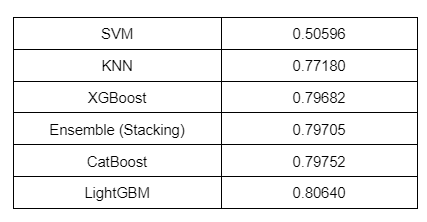
\includegraphics[scale=0.5]{spaceship_log.png}}
    \caption{Log Submission Dataset Spaceship}
    \label{spaceship_log}
\end{figure}

Pada ``Fig. ~\ref{spaceship_log}'', dapat dilakukan inferensi jika model klasifikasi berbasis tree seperti LGBMClassifier, CatBoostClassifier, XGB memiliki performa yang lebih baik. 
Model-model tersebut diperlakukan sama dengan standard scaler dan menggunakan gridsearch untuk hyperparameter tuning dan StratifiedKFold, yang membedakan hanya pada bagian classifiernya saja. 
Untuk algoritma KNNClassifier, proses training dengan menggunakan PCA cenderung memperoleh hasil yang lebih baik. Dalam klasifikasi dataset Spaceship Titanic, model 
LightGBM dengan dengan data hasil pemrosesan awal menggunakan standard scaler memberikan performa paling optimal jika dibandingkan dengan algoritma klasifikasi lainnya.

\subsection{Dataset Bank Churn}
Pemrosesan awal dataset Bank Churn dilakukan dengan melakukan tiga tahapan utama: scaling, encoding, dan feature engineering. Tahapan imputasi tidak dilakukan karena dataset tidak memiliki missing value. 
Scaling data dilakukan dengan menggunakan standard scaling (ST). Encoding pada dataset menggunakan one-hot encoding pada fitur Geography dan Gender. Tahap akhir, dilakukan proses feature engineering pada dataset surname. 
Dari proses tersebut, didapatkan sebuah clean dataset dengan tipe data numerik yang akan diujikan pada beberapa model.

Pada percobaan menggunakan model klasifikasi Gaussian Naive Bayes (GNBClassifier), diperoleh akurasi sebesar 0.80 dengan menggunakan metode evaluasi cross-validation. Ketika menambahkan Principal Component Analysis (PCA) dengan nilai 
n\_components = 10, diperoleh akurasi sebesar 0.81. Penggunaan PCA memperlihatkan nilai akurasi yang sedikit lebih baik pada model ini. 

Pada percobaan menggunakan model Gradient Boost Algorithm (XGBClassifier), dengan nilai PCA yang sama, diperoleh hasil  evaluasi 0.860. Ketika n\_components = 13, nilai evaluasi meningkat menjadi 0.865. 
Berdasarkan percobaan ini, dapat disimpulkan bahwa PCA dengan n\_components yang lebih sedikit kurang relevan digunakan dalam XGBClassifier. Untuk meningkatkan performa, model ini ditambahkan 
hyperparameter tuning dengan menggunakan gridsearchCV. Hasilnya nilai evaluasi yang diperoleh adalah sebesar 0.868. Penggunaan hyperparameter yang kurang cocok pada model ini adalah subsample karena dapat berpengaruh pada jumlah sampel dalam pelatihan.

Model KNN menggunakan PCA n\_components=0.1. Pada model ini, nilai K yang digunakan adalah 20 dan parameter yang digunakan adalah weights dan metrics. 
Dengan metric ROC-AUC, diperoleh nilai evaluasi 0.87, sedangkan dengan gridsearch diperoleh akurasi 0.85. Model KNN menunjukkan parameter weight berupa distance dan metrics. Model KNN dengan manhattan distance 
menghasilkan nilai akurasi yang lebih baik.

LBGMClassifier menghasilkan nilai relatif lebih tinggi dibandingkan dengan model lainnya untuk dataset ini. Model ini menggunakan gridsearch dengan parameter 
n\_estimators, learning\_rate, dan max\_depth. Penggunaan parameter subsample awalnya digunakan, akan tetapi hasil lebih baik ketika tidak menggunakan sub sample. 
Evaluasi dilakukan dengan ROC-AUC dan menghasilkan nilai evaluasi 0.90 dan evaluasi menggunakan randomized search diperoleh 0.898, dari hasil gridsearch, f1-score yang 
diperoleh sebesar 0.87 dan cross-validation menghasilkan skor 0.899.

Penggunaan Model CatBoostClassifier menghasilkan nilai evaluasi yang serupa dengan LGBMClassifier.. Model ini menggunakan GridSearchCV dengan parameter iterations, 
learning\_rate, depth, l2\_leaf\_reg, border\_count, dan loss\_function. Evaluasi dilakukan dengan menggunakan ROC-AUC dan cross-validation. Evaluasi menggunakan ROC-AUC 
menghasilkan skor sebesar 0.90, sedangkan dengan menggunakan cross-validation diperoleh skor sebesar 0.899.

\begin{figure}[htbp]
    \centerline{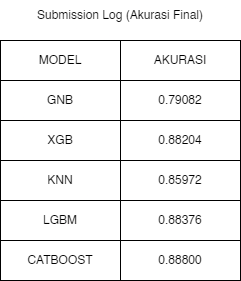
\includegraphics[scale=0.5]{churn_log.png}}
    \caption{Log Submission Dataset Bank Churn}
    \label{churn_log}
\end{figure}

Pada ``Fig. ~\ref{churn_log}'', dapat dilakukan inferensi jika model klasifikasi berbasis tree seperti LGBMClassifier dan CatBoostClassifier memiliki performa yang lebih baik. Untuk algoritma klasifikasi 
GaussianNB dan KNNClassifier, proses training dengan menggunakan PCA cenderung memperoleh hasil yang lebih baik. Dalam klasifikasi dataset Bank Churn, model CatBoostClassifier dengan dengan data hasil pemrosesan awal 
menggunakan min-max scaling (MM) memberikan performa paling optimal jika dibandingkan dengan algoritma klasifikasi lainnya.

\subsection{Dataset Horse Health}
Pada tahap preprocessing, yang dilakukan adalah beberapa langkah preprocessing dan feature engineering. Pertama, beberapa kolom kategorikal diencoding menggunakan LabelEncoder dan OneHotEncoder untuk mengubah nilai kategorikal menjadi numerik. 
Nilai tertentu dalam kolom seperti "pain", "peristalsis", "rectal\_exam\_feces", dan "nasogastric\_reflux" diganti untuk menyederhanakan kategori. Selanjutnya, nilai yang hilang dalam beberapa kolom diisi dengan nilai default dan di-mapping ke nilai numerik yang sesuai. 
Kolom "lesion\_3" dihapus karena dianggap tidak diperlukan. Feature engineering dilakukan dengan mengubah kolom "lesion\_2" menjadi biner dan membuat fitur baru "abs\_rectal\_temp" sebagai nilai absolut dari selisih antara "rectal\_temp" dan 37.8, kemudian kolom 
"rectal\_temp" dihapus. Langkah-langkah ini dilakukan untuk memastikan data dalam format yang sesuai untuk digunakan dalam model machine learning, dengan menangani nilai yang hilang, mengubah fitur kategorikal menjadi numerik, dan melakukan features engineering untuk meningkatkan kualitas data.

Setelah tahap preprocessing, setiap algoritma dalam model machine learning mengalami serangkaian langkah yang berbeda untuk mencapai performa terbaiknya. Algoritma LightGBM memanfaatkan teknik SMOTE untuk menangani ketidakseimbangan kelas sebelum melakukan pemodelan, 
awalnya mencapai akurasi sebesar 0.79. Setelah optimasi hyperparameter menggunakan GridSearch yang menghasilkan parameter terbaik {'learning\_rate': 0.2, 'min\_child\_samples': 20, 'n\_estimators': 500, 'num\_leaves': 70}, akurasi meningkat menjadi 0.81. 
CatBoost menggunakan class weights untuk menangani ketidakseimbangan kelas, mencapai akurasi 0.72 tanpa optimasi tambahan. RandomForest juga menggunakan class weights dengan akurasi awal 0.72, tetapi setelah optimasi hyperparameter 
dengan GridSearchCV, akurasi sedikit naik menjadi 0.73 dengan parameter terbaik {'bootstrap': True, 'max\_depth': 10, 'min\_samples\_leaf': 1, 'min\_samples\_split': 2, 'n\_estimators': 100}

Sebelum pemodelan dengan SVM, data dinormalisasi menggunakan MinMaxScaler, menghasilkan akurasi awal sebesar 0.49, menunjukkan bahwa normalisasi saja tidak cukup untuk meningkatkan performa model ini. XGBoost, seperti LightGBM, menggunakan SMOTE untuk menangani 
ketidakseimbangan kelas dan mencapai akurasi awal sebesar 0.77. Setelah optimasi hyperparameter menggunakan GridSearchCV dengan parameter terbaik {'colsample\_bytree': 0.3, 'learning\_rate': 0.2, 'max\_depth': 7, 'n\_estimators': 200}, akurasi meningkat menjadi 0.79. 
Decision Tree menggunakan MinMaxScaler untuk normalisasi dan class weights, mencapai akurasi awal 0.57. Setelah optimasi hyperparameter menggunakan GridSearchCV dengan parameter terbaik {'criterion': 'gini', 'max\_depth': None, 'min\_samples\_leaf': 10, 'min\_samples\_split': 2}, 
akurasi meningkat menjadi 0.64.

K-Nearest Neighbors (KNN) menggunakan MinMaxScaler untuk normalisasi dan SMOTE untuk menangani ketidakseimbangan kelas, mencapai akurasi awal sebesar 0.63. Setelah optimasi hyperparameter menggunakan GridSearchCV dengan parameter terbaik 
{'metric': 'manhattan', 'n\_neighbors': 3, 'weights': 'distance'}, akurasi sedikit meningkat menjadi 0.64. Naive Bayes menggunakan StandardScaler untuk standarisasi data dan SMOTE sebelum pemodelan, 
menghasilkan akurasi awal sebesar 0.62. Setelah optimasi hyperparameter menggunakan GridSearchCV dengan parameter terbaik {'var\_smoothing': 1e-05}, akurasi berada di angka 0.68. Nilai ini dapat dilihat pada ``Fig. ~\ref{horse_log}''

\begin{figure}[htbp]
    \centerline{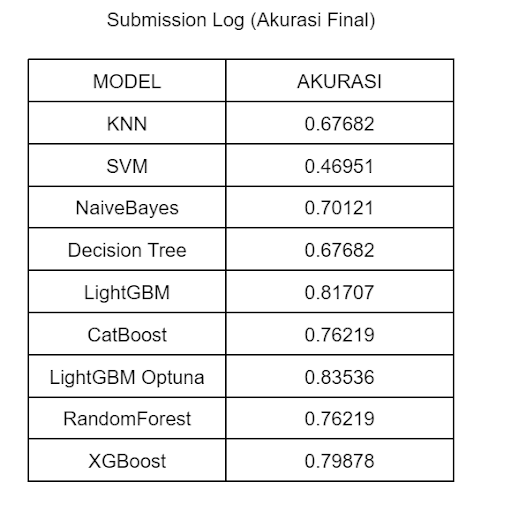
\includegraphics[scale=0.4]{horse_log.png}}
    \caption{Log Submission Dataset Horse Health}
    \label{horse_log}
\end{figure}

\subsection{Dataset Keep-it-Dry}

Pemrosesan awal dataset Keep-it-Dry dilakukan dengan melakukan tiga tahapan utama: imputasi, scaling dan encoding, serta imbalance handling. Pada tahapan imputasi, digunakan dua teknik imputasi dengan agregasi data berdasarkan product\_code: K-Nearest Neighbour Imputation (KI) dan Iterative Imputation (II). 
Proses scaling untuk data kontinu dengan menggunakan min-max scaling (MM), standard scaling (ST) dan robust scaling (RO) dan ketiganya menggunakan one-hot encoding. Proses imbalance handling dilakukan dengan teknik Random Over Sampler (ROS),
Random Under Sampler (RUS), SMOTE, SMOTENC, dan ADASYN. Dengan kombinasi terbentuk 16 clean dataset dengan beragam teknik pemrosesan awal yang akan diujikan pada tahap 
dataset selection untuk masing-masing model. Untuk setiap model yang digunakan, akan dilakukan dataset selection dengan melakukan testing ke-16 
clean dataset dengan menggunakan base model dengan penilaian berdasarkan F1-score.

\begin{figure}[htbp]
    \centerline{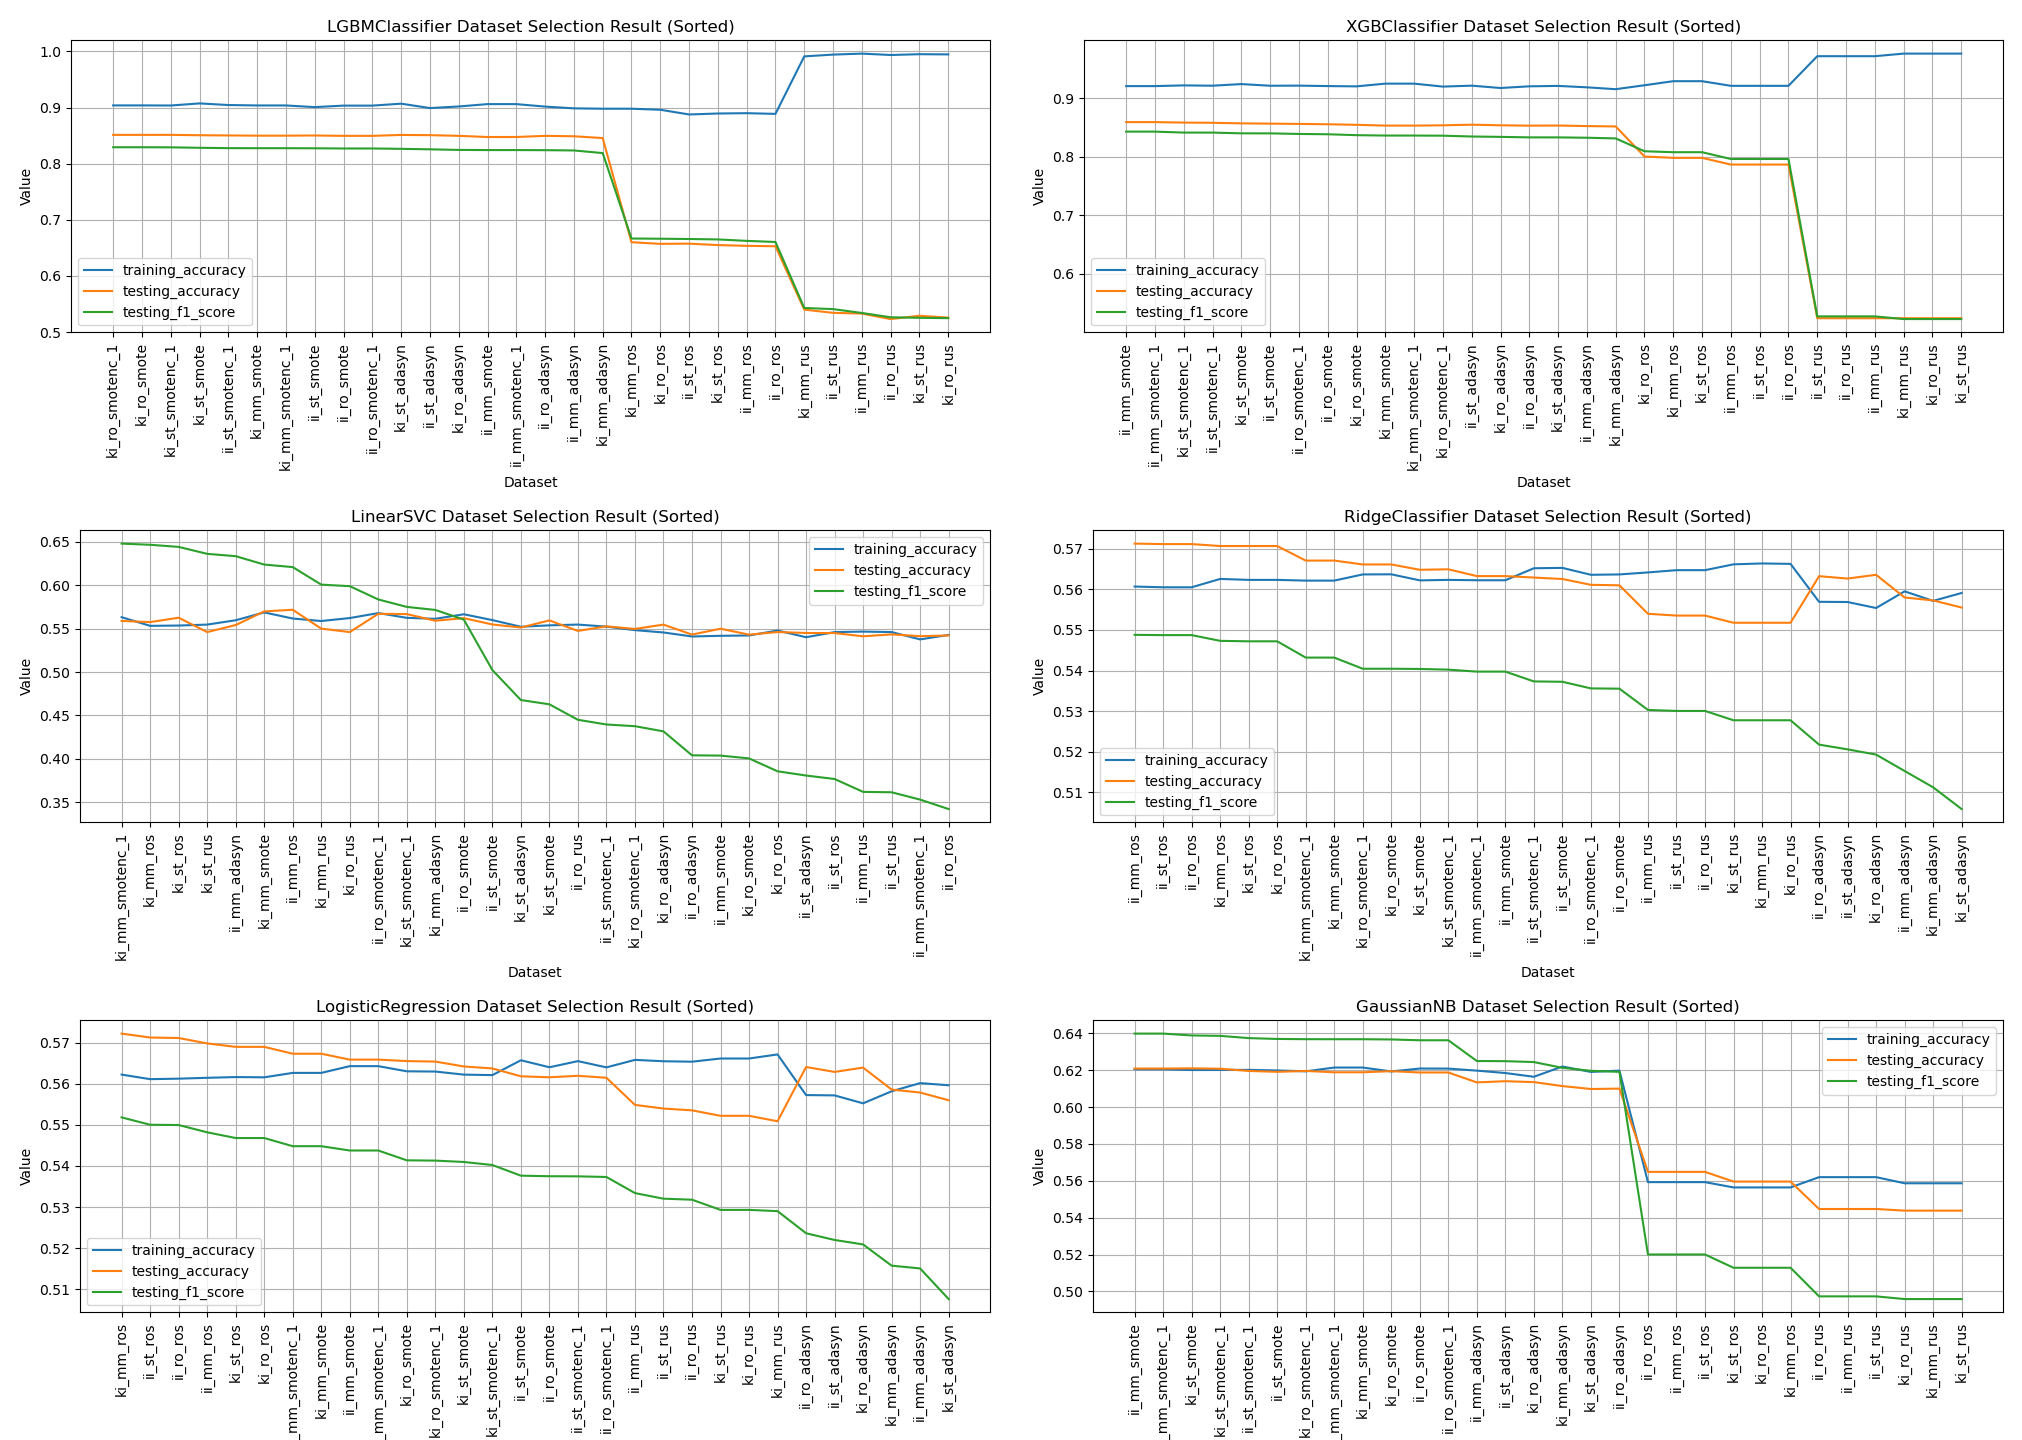
\includegraphics[width=\linewidth]{KID_Dataset_Selection.png}}
    \caption{Dataset Selection untuk Dataset Keep-it-Dry}
    \label{kid_datasetselection}
\end{figure}

Berdasarkan hasil dari dataset selection untuk berbagai model ``Fig. ~\ref{kid_datasetselection}'', teknik imbalance handling dengan SMOTE, SMOTENC, dan ADASYN (kode: \_*\_*smotenc\_1, \_*\_*smote, dan \_*\_*adasyn) 
memiliki performa yang lebih baik dalam proses klasifikasi pada training set dengan nilai F1-score yang tinggi jika dibandingkan dengan imbalance handling dengan ROS ataupun RUS 
(kode: \_*\_*ros dan \_*\_*rus). Akan tetapi, model yang dilatih dengan data resampling SMOTE, SMOTENC, dan ADASYN memberikan performa generalisasi yang jauh lebih buruk dari model yang dilatih dengan data 
resampling ROS dan RUS pada submission dataset. Oleh karenanya, dataset yang digunakan dalam proses hyperparameter tuning dan pelatihan model akan menggunakan dataset hasil resampling ROS atau RUS dengan nilai 
F1-score terbaik. Terlihat pula jika tree-based classifier seperti LGBMClassifier dan XGBClassifier memiliki rata-rata testing F1-score untuk proses dataset selection yang lebih baik.

Dari hasil data selection, selanjutnya adalah proses training dengan dataset yang menawarkan F1-score tertinggi. Sebagai bahan komparasi lanjutan, dilakukan pula training dengan dataset hasil resample ROS dan RUS. 
Proses Principal Component Analysis (PCA) diaplikasikan untuk meningkatkan performa generalisasi model. PCA dilakukan dengan menggunakan nilai variabel 
‘n\_components’ yang optimal untuk masing-masing base model dengan penilaian F1-score secara iteratif untuk rentang nilai n\_components [10, 23]. Proses roses training dijalankan bersamaan dengan proses 
hyperparameter tuning dengan validation data sebesar 75\% dari total training data. Untuk meningkatkan performa generalisasi model pada unseen data, digunakan pula 
cross-validation dengan folds sebanyak 5. Dengan best estimator yang didapatkan melalui hyperparameter tuning dengan cross-validation ini, dilakukan prediksi data submission.

\begin{figure}[htbp]
    \centerline{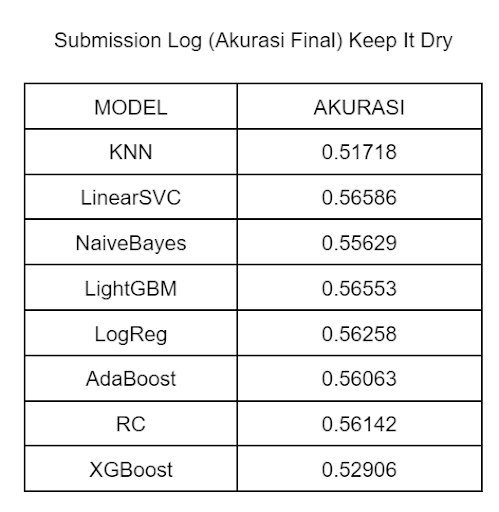
\includegraphics[scale=0.4]{kid_log.png}}
    \caption{Log Submission Dataset Keep-it-Dry}
    \label{kid_log}
\end{figure}

Terlihat pada ``Fig. ~\ref{kid_log}'', hasil akurasi pada data submission aktual menandakan adanya perbedaan antara testing F1-score dengan actual score. Model klasifikasi berbasis tree seperti XGBClassifier dan LGBMClassifier 
mengindikasikan adanya overfit pada data submission, bahkan setelah dilakukan hyperparameter tuning dengan cross-validation. Melalui retraining dan resubmission menggunakan dataset dengan testing F1-score yang lebih rendah (RUS-resampled), 
XGBClassifier dan LGBMClassifier justru memberikan hasil akurasi yang lebih baik pada data submission. Di sisi lain, model klasifikasi linear dengan regularisasi L2 seperti RidgeClassifier (RC)  dan LogisticRegression (LR) serta kernelized 
Linear SVM Classifier (LinearSVC), dengan testing F1-score yang lebih buruk dibandingkan XGBClassifier dan LGBMClassifier, mampu memberikan actual score data submission yang lebih baik. Hal yang sama juga berlaku untuk model klasifikasi Gaussian Naive-Bayes 
(GaussianNB) dan K-Nearest Neighbors (KNNClassifier). Dari hasil submission, terlihat jika model RC, LR, LinearSVC, GaussianNB dan KNNClassifier yang dilatih dengan dataset ROS-resampled memberikan performa aktual yang lebih baik pada data submission jika 
dibandingkan dengan dataset hasil synthetic resampling (SMOTE/SMOTENC/ADASYN).

Dari ``Fig. ~\ref{kid_log}'', dapat dilakukan inferensi jika model klasifikasi berbasis tree mampu memberikan performa yang lebih baik dengan melakukan training pada data dengan RUS-resampling dan PCA, membantu mengurangi dampak overfitting pada unseen data. 
Untuk algoritma klasifikasi RC, LR, LinearSVC, GaussianNB dan KNNClassifier, proses training pada data dengan ROS-resampling dan PCA memberikan performa yang lebih baik secara keseluruhan jika dibandingkan dengan algoritma klasifikasi berbasis tree. 
Dalam klasifikasi dataset Keep-it-Dry, model LinearSVC dengan hyperparameter {'C': 4.641588833612777, 'loss': 'squared\_hinge', 'penalty': 'l2'} dengan data hasil pemrosesan awal menggunakan robust scaling (RO) dan ROS-resampling memberikan performa paling optimal 
jika dibandingkan dengan algoritma klasifikasi lainnya. Dengan teknik pemrosesan awal yang sama, RC dan LR dengan hyperparameter tuning menggunakan Grid Search dan Cross-Validation juga memberikan performa yang baik setelah LinearSVC.

\section{Simpulan}
Pada Proyek Akhir  ini, kami mengeksplorasi sejumlah teknik untuk menangani ketidakseimbangan kelas dan proses resampling data dengan tujuan meningkatkan kinerja model klasifikasi. Kami mengevaluasi serta membandingkan teknik-teknik seperti 
Synthetic Minority Over-sampling Technique (SMOTE), SMOTE for Nominal and Continuous features (SMOTENC), Adaptive Synthetic Sampling (ADASYN), Random Over Sampling (ROS), dan Random Under Sampling (RUS). Temuan penelitian menunjukkan bahwa meskipun 
teknik SMOTE, SMOTENC, dan ADASYN mampu menghasilkan kinerja yang baik pada data pelatihan, namun cenderung mengalami overfitting pada data pengujian. Sebaliknya, teknik ROS dan RUS menunjukkan performa yang lebih konsisten dan unggul pada data pengujian, sehingga 
lebih kami pilih untuk digunakan dalam tahap tuning hyperparameter dan pelatihan model.

Penerapan Principal Component Analysis (PCA) juga terbukti efektif dalam meningkatkan kinerja generalisasi model dengan mengurangi dimensi data dan mengatasi masalah multikolinearitas. PCA membantu model fokus pada komponen yang paling signifikan, 
yang pada akhirnya meningkatkan akurasi prediksi. PCA digabungkan dengan berbagai model klasifikasi dan memberikan hasil yang positif, menunjukkan pentingnya teknik ini dalam proses preprocessing data sebelum pelatihan model.

Model klasifikasi yang kami uji meliputi algoritma berbasis pohon keputusan seperti Extreme Gradient Boosting (XGBClassifier) dan Light Gradient Boosting Machine (LGBMClassifier), serta model linear seperti RidgeClassifier, LogisticRegression, 
dan Linear Support Vector Classification (LinearSVC). Hasil eksperimen menunjukkan bahwa model berbasis pohon keputusan cenderung mengalami overfitting, sementara model linear menunjukkan performa yang lebih stabil dan dapat diandalkan 
pada data pengujian. Hal ini menekankan pentingnya pemilihan model yang sesuai berdasarkan karakteristik dataset yang digunakan.

Selain itu, kami juga menguji metode ensemble seperti Stacking, yang menghasilkan kinerja yang kompetitif namun rentan terhadap overfitting jika tidak ditangani dengan benar. Pemilihan dan kombinasi model dalam ensemble harus dilakukan dengan 
hati-hati untuk memastikan generalisasi yang baik pada data pengujian.

Secara keseluruhan, proyek ini menunjukkan bahwa penanganan ketidakseimbangan kelas, penerapan PCA, dan penggunaan metode ensemble dapat signifikan meningkatkan kinerja model klasifikasi. Implementasi teknik resampling yang 
tepat dan tuning hyperparameter yang cermat adalah langkah penting dalam pengembangan model yang akurat dan robust. Proyek ini memberikan wawasan berharga bagi praktisi dalam mengembangkan model klasifikasi yang efektif.

\section{Kode Program dan Kontribusi}
\begin{itemize}
    \item Kode program yang digunakan dalam studi komparasi algoritma klasifikasi \textit{Supervised Learning} pada artikel ini dapatdiakses pada tautan berikut: https://github.com/rayhanegar/Bntr-y-lg-diskusi
    \item Laporan kontribusi dan laporan kemajuan selama proses studi komparasi algoritma klasifikasi \textit{Supervised Learning} dapat diakses pada tautan berikut: https://s.ub.ac.id/progressppmdfinal
\end{itemize}

\begin{thebibliography}{00}
\bibitem{b1} GeeksforGeeks, “Machine Learning Tutorial,” GeeksforGeeks, May 30, 2018. https://www.geeksforgeeks.org/machine-learning.
\bibitem{b2} “Machine Learning,” Coursera, 2018. https://www.coursera.org/specializations/machine-learning-introduction.
\bibitem{b3} Machine Learning, “Machine Learning,” IEEE DataPort, 2024. https://ieee-dataport.org/taxonomy/term/2005/all?page=2.
\bibitem{b4} Shai Shalev-Shwartz and Shai Ben-David, Understanding machine learning: From foundations to algorithms. Cambridge Etc: Cambridge University Press, 2014.
\bibitem{b5} F. Maymí and S. Lathrop, ''AI in Cyberspace: Beyond the Hype,'' 2024.
\bibitem{b6} V. V. Putri Wibowo, Z. Rustam, and J. Pandelaki, ''Classification of Brain Tumor Using K-Nearest Neighbor-Genetic Algorithm and Support Vector Machine-Genetic Algorithm Methods,'' in 2021 International Conference on Decision Aid Sciences and Application, Sakheer, Bahrain: IEEE, Dec. 2021, pp. 1077--1081. doi: 10.1109/DASA53625.2021.9682341.
\bibitem{b7} N. F. B. M. Noor, H. S. Sipail, N. Ahmad, and N. M. Noor, ''Covid-19 Severity Classification Using Supervised Learning Approach,'' in 2021 IEEE National Biomedical Engineering Conference, Kuala Lumpur, Malaysia: IEEE, Nov. 2021, pp. 151--156. doi: 10.1109/NBEC53282.2021.9618747.
\bibitem{b8} A. P. Pawlovsky and H. Matsuhashi, ''The use of a novel genetic algorithm in component selection for a kNN method for breast cancer prognosis,'' in 2017 Global Medical Engineering Physics Exchanges/Pan American Health Care Exchanges, Tuxtla-Gutierrez, Mexico: IEEE, Mar. 2017, pp. 1--5. doi: 10.1109/GMEPE-PAHCE.2017.7972084.
\bibitem{b9} A. C. Müller and S. Guido, Introduction to Machine Learning with Python: A Guide for Data Scientists. Beijing: O'reilly, 2017.
\bibitem{b10} K. Kim, ''Normalized class coherence change-based k NN for classification of imbalanced data,'' Pattern Recognition, vol. 120, p. 108126, Dec. 2021, doi: 10.1016/j.patcog.2021.108126.
\bibitem{b11} K. Yuk Carrie Lin, ''Optimizing variable selection and neighbourhood size in the K-nearest neighbour algorithm,'' Computers and Industrial Engineering, vol. 191, p. 110142, May 2024, doi: 10.1016/j.cie.2024.110142.
\bibitem{b12} S. Zhang, D. Cheng, Z. Deng, M. Zong, and X. Deng, ''A novel k NN algorithm with data-driven k parameter computation,'' Pattern Recognition Letters, vol. 109, pp. 44--54, Jul. 2018, doi: 10.1016/j.patrec.2017.09.036.
\bibitem{b13} A. Rokem and K. Kay, ''Fractional ridge regression: a fast, interpretable reparameterization of ridge regression,'' GigaScience, vol. 9, no. 12, p. giaa133, Nov. 2020, doi: 10.1093/gigascience/giaa133.
\bibitem{b14} B. Akturk, U. Beyaztas, H. L. Shang, and A. Mandal, ''Robust functional logistic regression,'' Adv Data Anal Classif, Feb. 2024, doi: 10.1007/s11634-023-00577-z.
\bibitem{b15} M. Arifuzzaman, Md. R. Hasan, T. J. Toma, S. B. Hassan, and A. K. Paul, ''An Advanced Decision Tree-Based Deep Neural Network in Nonlinear Data Classification,'' Technologies, vol. 11, no. 1, p. 24, Feb. 2023, doi: 10.3390/technologies11010024.
\bibitem{b16} F. Aaboub, H. Chamlal, and T. Ouaderhman, ''Analysis of the prediction performance of decision tree-based algorithms,'' in 2023 International Conference on Decision Aid Sciences and Applications (DASA), Annaba, Algeria: IEEE, Sep. 2023, pp. 7--11. doi: 10.1109/DASA59624.2023.10286809.
\bibitem{b17} R. G. Mantovani, T. Horvath, R. Cerri, J. Vanschoren, and A. C. P. L. F. De Carvalho, ''Hyper-Parameter Tuning of a Decision Tree Induction Algorithm,'' in 2016 5th Brazilian Conference on Intelligent Systems (BRACIS), Recife: IEEE, Oct. 2016, pp. 37--42. doi: 10.1109/BRACIS.2016.018.
\bibitem{b18} Y.-C. Zhang and L. Sakhanenko, "The naive Bayes classifier for functional data," Department of Statistics and Probability, Michigan State University, East Lansing, MI, USA, Accepted April 27, 2019.
\bibitem{b19} A. Khajenezhad, M. A. Bashiri, and H. Beigy, "A distributed density estimation algorithm and its application to naive Bayes classification," Sharif Intelligent Systems Laboratory, Department of Computer Engineering, Sharif University of Technology, Tehran, Iran, Accepted October 20, 2020.
\bibitem{b20} N. Guenther dan M. Schonlau, "Support vector machines," The Stata Journal, vol. 16, no. 4, pp. 917--937, 2016.
\bibitem{b21} E. Osuna, R. Freund, dan F. Girosi, "An improved training algorithm for support vector machines," in Proceedings of IEEE, 1997, pp. 252--1723.
\bibitem{b22} C. Cortes dan V. Vapnik, "Support-vector networks," Machine Learning, vol. 20, pp. 273-297, 1995.
\bibitem{b23} N. Settouti, M. El Habib Daho, M. E. Amine Lazouni, and M. A. Chikh, "Random forest in semi-supervised learning (Co-Forest)," in 2013 8th International Workshop on Systems, Signal Processing and their Applications (WoSSPA), Algiers, Algeria, 2013, pp. 326-329, doi: 10.1109/WoSSPA.2013.6602385.
\bibitem{b24} P. S. Akash, M. E. Kadir, A. A. Ali, M. N. Ahad Tawhid, and M. Shoyaib, "Introducing Confidence as a Weight in Random Forest," in 2019 International Conference on Robotics, Electrical and Signal Processing Techniques (ICREST), Dhaka, Bangladesh, 2019, pp. 611-616, doi: 10.1109/ICREST.2019.8644396.
\bibitem{b25} C. Bentéjac, A. Csörgő, and G. Martínez-Muñoz, "A Comparative Analysis of XGBoost," Preprint, Nov. 2019.
\bibitem{b26} T. Chen and C. Guestrin, "XGBoost: A Scalable Tree Boosting System," in Proceedings of the 22nd ACM SIGKDD International Conference on Knowledge Discovery and Data Mining (KDD '16), New York, NY, USA, 2016, pp. 785–794, doi: 10.1145/2939672.2939785.
\bibitem{b27} P. Zhang, Y. Jia, and Y. Shang, "Research and application of XGBoost in imbalanced data," International Journal of Distributed Sensor Networks, vol. 18, no. 6, 2022, doi: 10.1177/15501329221106935.
\bibitem{b28} C. P. Ananda, ''Machine Learning Untuk Prediksi Gaya Hidup Berdasarkan Socioeconomic Status Ses Menggunakan Algoritma Catboost Studi Kasus: Mahasiswa UIN Jakarta'', Bachelor's thesis, Fakultas Sains dan Teknologi UIN Syarif Hidayatullah Jakarta
\bibitem{b29} R. Sanjeetha, A. Raj, K. Saivenu, M. I. Ahmed, B. Sathvik, A. Kanavalli, ''Detection and mitigation of botnet based DDoS attacks using catboost machine learning algorithm in SDN environment,'' International Journal of Advanced Technology and Engineering Exploration, vol. 8, no. 76, p. 445., 2021.
\bibitem{b30} Rizky, P. S., Hirzi, R. H., Hidayaturrohman, U. (2022). Perbandingan Metode LightGBM dan XGBoost dalam Menangani Data dengan Kelas Tidak Seimbang. J Statistika: Jurnal Ilmiah Teori dan Aplikasi Statistika, 15(2), 228-236.
\bibitem{b31} Shehadeh, A., Alshboul, O., Al Mamlook, R. E., Hamedat, O. (2021). Machine learning models for predicting the residual value of heavy construction equipment: An evaluation of modified decision tree, LightGBM, and XGBoost regression. Automation in Construction, 129, 103827.
\bibitem{b32} Nugraha, A. F., Aziza, R. F. A., Pristyanto, Y. (2022). Penerapan metode stacking dan random forest untuk meningkatkan kinerja klasifikasi pada proses deteksi web phishing. Jurnal Infomedia: Teknik Informatika, Multimedia, dan Jaringan, 7(1), 39-44.
\bibitem{b33} Sanjaya, J., Renata, E., Budiman, V. E., Anderson, F., Ayub, M. (2020). Prediksi Kelalaian Pinjaman bank Menggunakan random forest Dan adaptive boosting. Jurnal Teknik Informatika dan Sistem Informasi, 6(1).
\bibitem{b34} Pandey, P., Prabhakar, R. (2016, August). An analysis of machine learning techniques (J48 and AdaBoost)-for classification. In 2016 1st India International Conference on Information Processing (IICIP) (pp. 1-6). IEEE. 
\bibitem{b35} Little, R.J.A., Rubin, D.B. (2002). "Statistical Analysis with Missing Data." John Wiley \% Sons.
\bibitem{b36} Witten, I.H., Frank, E., \& Hall, M.A. (2011). "Data Mining: Practical Machine Learning Tools and Techniques." Morgan Kaufmann.
\bibitem{b37} Han, J., Kamber, M., \& Pei, J. (2011). "Data Mining: Concepts and Techniques." Morgan Kaufmann.
\bibitem{b38} Chawla, N.V., Japkowicz, N., \& Kotcz, A. (2004). "Editorial: Special Issue on Learning from Imbalanced Data Sets." ACM SIGKDD Explorations Newsletter.
\bibitem{b39} Jolliffe, I.T., \& Cadima, J. (2016). "Principal component analysis: a review and recent developments." Philosophical Transactions of the Royal Society A.
\bibitem{b40} I. S. Mangkunegara and P. Purwono, "Analysis of DNA Sequence Classification Using SVM Model with Hyperparameter Tuning Grid Search CV," 2022 IEEE International Conference on Cybernetics and Computational Intelligence (CyberneticsCom), Malang, Indonesia, 2022.
\bibitem{b41} Anjan, G.S.K.; Kumar Verma, A.; Radhika, S. K-Nearest neighbors and grid search CV based real time fault monitoring system for industries. In Proceedings of the 2019 IEEE 5th International Conference for Convergence in Technology, I2CT 2019, Bombay, India, 29–31 March 2019; p. 5.
\bibitem{b42} T. Yan, S. L. Shen, A. Zhou, and X.-S. Chen, “Prediction of geological characteristics from shield operational parameters using integrating grid search and K-fold cross validation into stacking classification algorithm,”, 2022
\bibitem{b43} K. R. Singh, K. P. Neethu, K. Madhurekaa, A. Harita, and P. Mohan, “Parallel SVM model for forest fire prediction,”, 2021.
\bibitem{b44} Polipireddy Srinivas, Rahul Katarya, “hyOPTXg: OPTUNA hyper-parameter optimization framework for predicting cardiovascular disease using XGBoost,” Biomedical Signal Processing and Control, Volume 73, 2022.
\bibitem{b45} Akiba, T., Sano, S., Yanase, T., Ogino, Y., \& Ohta, N. (2019, Juni). “Optuna: A distributed hyperparameter optimization framework,” In Proceedings of the 25th ACM SIGKDD International Conference on Knowledge Discovery and Data Mining
\bibitem{b46} D. Marutho, "Perbandingan Metode Naïve Bayes, KNN, Decision Tree pada Laporan Water Level Jakarta," Infokam, vol. II, no. XV, pp. SEPTEMBER, 2019.
\bibitem{b47} S. Lonang, A. Yudhana, and M. K. Biddinika, "Analisis Komparatif Kinerja Algoritma Machine Learning untuk Deteksi Stunting," J. Media Informatika Budidarma, vol. 7, no. 4, pp. 2109-2117, Oct. 2023.
\bibitem{b48} I. J. Sokolova and G. Lapin, "A unified approach to evaluation metrics for binary classification tasks," IEEE Transactions on Pattern Analysis and Machine Intelligence, vol. 31, no. 12, pp. 2274-2289, Dec. 2009. DOI: 10.1109/TPAMI.2009.113
\bibitem{b49} R. Caruana et al., "Beyond accuracy, precision, and recall: The quest for a comprehensive performance metric in machine learning," in Proceedings of the 21th ACM SIGKDD International Conference on Knowledge Discovery and Data Mining, New York, NY, USA, Aug. 2014, pp. 239-248. DOI: 10.1145/2670495.2670547
\bibitem{b50} D. Stone, "Cross-validation: A simple and powerful method for evaluation of learning algorithms," Journal of the American Statistical Association, vol. 79, no. 387, pp. 575-583, Sep. 1974.

\end{thebibliography}
\vspace{12pt}

\end{document}
